\documentclass[conference]{IEEEtran}
\IEEEoverridecommandlockouts
\usepackage{cite}
\usepackage{amsmath,amssymb,amsfonts}
\usepackage{algorithmic}
\usepackage{graphicx}
\usepackage{textcomp}
\usepackage{xcolor}
\usepackage{float}
\usepackage{rotating}

\def\BibTeX{{\rm B\kern-.05em{\sc i\kern-.025em b}\kern-.08em
    T\kern-.1667em\lower.7ex\hbox{E}\kern-.125emX}}

\begin{document}
\sloppy

\title{AquaOptima: Apply Evolutionary Algorithm and Particle Swarm Optimization in Virtual Largemouth Bass Aquaculture\\}

\author{
\IEEEauthorblockN{Leon Hoang}
\IEEEauthorblockA{\textit{Tickle College of Engineering} \\
University of Tennessee\\
Knoxville, USA\\
phoang5@vols.utk.edu}
\and
\IEEEauthorblockN{Ahmed Ghazi}
\IEEEauthorblockA{\textit{Tickle College of Engineering} \\
University of Tennessee\\
Knoxville, USA\\
aghazi2@vols.utk.edu}
}

\maketitle

\begin{abstract}
\normalfont
This report investigates the optimization of Largemouth Bass (\textit{Micropterus salmoides}) aquaculture policies using a custom biologically-inspired simulation framework, AquaOptima. The project addresses the critical challenge of maintaining high survival rates and optimal fish health while minimizing economic overhead. AquaOptima employs Particle Swarm Optimization (PSO) to create a biologically realistic 3D agent-based model of fish behavior, capturing complex dynamics such as foraging, oxygen-seeking, disease avoidance, and intracohort cannibalism. To discover optimal management strategies, an Evolutionary Algorithm (EA) evaluates and mutates policies governing food, probiotic, and oxygen distribution. Given the high susceptibility of these populations to bacterial pathogens and rapid environmental shifts, precise computational resource management is crucial. Across 10 independent timelines and 20 generations, the EA successfully navigated the exploration-exploitation trade-off, converging on policies that eliminate starvation and suffocation without exceeding strict budgetary constraints. Ultimately, the results demonstrate the efficacy of combining PSO-driven agent models with evolutionary computation to reliably solve multi-objective physical phenomena in modern aquaculture systems.
\end{abstract}

\begin{IEEEkeywords}
Particle Swarm Optimization, Evolutionary Algorithms, Agent-Based Modeling, Aquaculture, Micropterus salmoides
\end{IEEEkeywords}

\section{Introduction and Motivation}

\subsection{Project Goal}
Aquaculture operations face constant pressure to maximize yield while adhering to strict economic and environmental constraints. The overarching goal of this project is to develop an intelligent, automated management system capable of optimizing resource distribution---specifically food, probiotics, and oxygen---for Largemouth Bass.

\subsection{Research Question}
The primary research question addressed in this study is: \textit{Can Evolutionary Algorithms (EA) be used to optimize the parameters of a complex, agent-based model (driven by Particle Swarm Optimization) to maximize the survival and health of a simulated fish population while minimizing operational costs?}

\subsection{Topic Significance and Algorithm Selection}
This topic is of particular interest because biological systems are highly sensitive to environmental factors. Largemouth Bass populations are prone to high mortality rates during specific seasons, are highly susceptible to bacterial pathogens, and exhibit natural intracohort cannibalism when starved. Standard mathematical models often fail to capture these localized, agent-level interactions. By utilizing bio-inspired computation---specifically PSO to simulate the swarm intelligence of the fish and EA to evolve the management policies---we can realistically simulate these physical phenomena and derive highly optimized, non-intuitive solutions that traditional optimization methods might miss.

\section{Related Work}
Agent-based modeling (ABM) and bio-inspired algorithms are increasingly utilized to understand complex biological systems. Previous works have established the efficacy of using agent-based modeling in fisheries and aquaculture, successfully simulating factors like dissolved oxygen levels, fish shoal behavior, and spatial management strategies \cite{smith2024}, \cite{doe2023}.

In the specific context of Largemouth Bass aquaculture, researchers have documented the severe environmental impacts of poor pond management \cite{zhang} and the distinct challenges of maintaining high survival rates across seasons \cite{vodianitskyi}. Disease management remains a massive hurdle, with extensive research dedicated to controlling mortality caused by bacterial pathogens like \textit{Columnaris} and \textit{Aeromonas} \cite{bowker}, \cite{wang2025}. To combat this, recent studies have proven the effectiveness of dietary probiotic supplementation (such as \textit{Lactobacillus reuteri}) to significantly boost fish immunity and metabolism \cite{li}. Furthermore, behavioral constraints, such as aggressive intracohort cannibalism driven by size disparity and starvation, are well-documented phenomena in Age-0 Largemouth Bass \cite{post}.

Computationally, Particle Swarm Optimization (PSO) has been a foundational bio-inspired algorithm since its introduction, modeling the social behavior of bird flocks and fish schools to optimize non-linear functions \cite{kennedy1995}. However, while existing research applies ABMs to observe fish, and uses PSO for general mathematical optimization, few studies bridge the gap.

\textbf{What this project does differently:} AquaOptima directly integrates biological reality with computational optimization. Instead of treating the fish as static data points, this project uses a modified PSO algorithm to simulate their real-time survival behaviors (schooling, fleeing hazards, foraging). It then wraps this highly volatile simulation in an Evolutionary Algorithm to evolve an external ``manager'' policy.

\section{Experimental Setup and Approach}
The experiment was constructed entirely within a custom Python framework, \texttt{AquaOptima}. The simulation relies on two distinct biologically-inspired algorithms operating in tandem.

\subsection{The Environment}
The simulation takes place in a 3D continuous pond space with dimensions of $180 \times 85 \times 50$ (width $\times$ height $\times$ depth). To establish a biologically realistic population, the initial fish count is calculated dynamically based on the pond's volume using a density scaling factor ($K = 0.55$) derived from standard intensive pond culture guidelines \cite{tidwell}:
\begin{equation}
\boxed{
InitialFish = \max\left(10, \left\lfloor K \times (W \times H \times D)^{\frac{1}{3}} \right\rfloor\right)
}
\end{equation}
For this specific pond volume, the simulation finalizes the initial population at 50 fish.

The environment operates on a complex, cyclic interaction model where physical objects and biological agents continuously influence each other:
\begin{itemize}
    \item \textbf{Consumption and Waste:} Fish consume dropped food, probiotics, and oxygen bubbles to replenish their physiological stats. As fish metabolize, they routinely produce sinking fecal waste, a primary driver of pond eutrophication \cite{zhang}.
    \item \textbf{Pollutant Transformation:} Uneaten food, expired probiotics, and accumulated fecal waste on the pond floor eventually decay into generic pollutants. Over time, these pollutants probabilistically transform into natural hazards (such as ammonia bubbles, disease zones, and parasites), benign plants, or new physical obstacles \cite{zhang}.
    \item \textbf{Environmental Hazards:} Water quality degradation introduces severe physiological penalties \cite{zhang}. Ammonia (NH3) hazards rapidly deplete fish oxygen and health by restricting respiratory efficiency. Furthermore, disease and parasite zones (simulating common bacterial pathogens like \textit{Columnaris} and \textit{Aeromonas}) severely drain fish immunity and induce long-term physiological decay \cite{bowker}, \cite{wang2025}. Unmitigated, these hazards can wipe out entire populations.
    \item \textbf{Mortality:} If a fish starves, suffocates, or succumbs to disease, its body will either sink or float. These decaying bodies act as massive, localized ammonia emitters before ultimately breaking down into dense pollutants, creating a deadly feedback loop in crowded spaces \cite{zhang}, \cite{bowker}.
    \item \textbf{Cannibalism:} We intentionally selected Largemouth Bass (\textit{Micropterus salmoides}) for this simulation because they exhibit highly aggressive intracohort cannibalism \cite{post}. This behavioral constraint adds an interesting layer to the experiment: severely starved fish act as natural enemies to their smaller cohort members. This introduces a complex predator-prey dynamic without requiring the computational overhead of rendering a completely separate predatory species. Successful cannibals directly remove competitors while gaining a massive fullness boost.
\end{itemize}

\subsection{PSO Agent Behavior}
The fish agents are driven by a modified PSO velocity update algorithm. Rather than seeking a single mathematical global minimum, each particle's (fish's) velocity vector is influenced by a dynamic weighting system based on its internal physiological state:
\begin{itemize}
    \item \textbf{Foraging:} Particles steer toward food, with the weight urgency scaling via an inverse square root of their fullness.
    \item \textbf{Survival:} Particles aggressively steer toward oxygen and probiotics when internal reserves fall below critical thresholds.
    \item \textbf{Avoidance:} High weights are assigned to fleeing high-density NH3 hazard zones and larger predatory fish to avoid intracohort cannibalism.
    \item \textbf{Schooling:} Standard PSO cognitive and social parameters balance selfish spacing with group schooling.
\end{itemize}

\subsection{Evolutionary Algorithm (EA) Setup}
The EA acts as the ``manager'' trying to keep the PSO swarm alive. It is important to clarify that biological reproduction (fish breeding) is not simulated due to the extreme computational complexity it would add to the existing physics engine, though it remains a strong potential avenue for future work. Instead, the evolutionary process is applied entirely to the controllable factors of the environment---specifically, the management \textit{policies}---rather than the highly stochastic, chaotic factors governing the biological and physical interactions of the pond. To accurately model and optimize this environment, the EA was structured with the following components:

\subsubsection{Parameters}
To ensure robust evaluation and statistical significance, the experiment parameters are defined as follows:
\begin{itemize}
    \item \textbf{Timelines:} 10 independent timelines. Each timeline acts as a separate, parallel run to mitigate the risk of poor initial randomization. The variance between timelines is driven by two factors: the randomized genotypes of the initial policy populations, and the highly chaotic outcomes stemming from the stochastic nature of the environment setup (e.g., random hazard spawns, unpredictable fish movement).
    \item \textbf{Generations:} 20 generations per timeline.
    \item \textbf{Population Size:} 20 candidate policies per generation.
    \item \textbf{Simulation Duration:} 30-day aquaculture period, where each time step represents 1 hour in the virtual simulation.
    \item \textbf{Budget Constraint:} Strict maximum budget of \$500. If a policy exhausts this budget before day 30, the simulation terminates early for that pond.
    \item \textbf{Resource Costs:} Food at \$0.10 per pellet, Probiotics at \$0.50 per pellet, and Oxygen pumping at \$1.50 per duration hour.
\end{itemize}

\subsubsection{Genotype}
The genotype represents a specific aquaculture policy consisting of 9 parameters, detailed in Table \ref{tab:genotype}.

\begin{table}[htbp]
\centering
\caption{Genotype Parameters, Ranges, and Mutations}
\label{tab:genotype}
\begin{tabular}{|p{0.25\linewidth}|p{0.65\linewidth}|}
\hline
\textbf{Resource} & \textbf{Parameters (Range) [Mutation Step]} \\ \hline
\textbf{Food} & Interval: 1--24h [$\pm$4h] \newline Quantity: 1--10 pellets [$\pm$2] \newline Location: Center or Random [Flip] \\ \hline
\textbf{Probiotics} & Interval: 12--168h [$\pm$1 index] \newline Quantity: 0--4 pellets [$\pm$1] \newline Location: Center or Random [Flip] \\ \hline
\textbf{Oxygen} & Interval: 1--24h [$\pm$4h] \newline Duration: 1--3h [$\pm$1h] \newline Location: Center or Random [Flip] \\ \hline
\end{tabular}
\end{table}

The EA utilizes a crossover rate of 80\% ($0.80$) and a mutation rate of 25\% ($0.25$). The high crossover rate of 80\% is specifically selected to help preserve and continuously recombine ``good genes'' (successful policy traits) within the highly chaotic and stochastic simulation environment. To counterbalance this high crossover and prevent premature convergence, the 25\% mutation rate allows for consistent exploration of the search space.

Mutation applies Gaussian perturbation for numeric intervals and quantities, and binary flips for categorical drop locations. Gaussian perturbation is explicitly chosen over uniform random replacement to prevent drastic, destructive changes to elite policies. By taking small, localized steps in the search space, it mitigates environmental noise while allowing the EA to safely fine-tune near-optimal solutions. For example, a highly successful food interval of 12 hours might mutate slightly to 16 or 8 hours, rather than jumping erratically to 1 hour and starving the population.

\subsubsection{Fitness Function}
The fitness function acts as the mathematical compass for the evolutionary algorithm, driving the swarm towards optimal multi-objective performance. The function automatically rejects any policy that exceeds the strict \$500 operational budget. For policies within the budget, it aggregates three normalized metrics (scaled from 0 to 1) into a single scalar value:

\begin{equation}
\boxed{
\begin{aligned}
Fitness ={} & 0.55 \times SurvivalRate \\
            & + 0.33 \times SavingRate \\
            & + 0.12 \times Healthiness
\end{aligned}
}
\end{equation}

Each term was explicitly weighted to reflect real-world aquaculture priorities:
\begin{itemize}
    \item \textbf{SurvivalRate (0.55):} The highest priority. It is calculated as the final percentage of the original fish population still alive at day 30. Keeping the population alive is the absolute prerequisite for any viable aquaculture business.
    \item \textbf{SavingRate (0.33):} The second priority. Calculated as the fraction of the \$500 budget remaining at the end of the simulation. This incentivizes the algorithm to find minimal-resource strategies rather than continually dumping expensive food and oxygen into the pond.
    \item \textbf{Healthiness (0.12):} The final priority. It measures the aggregate average internal physiological state of the surviving fish (e.g., immunity levels, starvation levels). This acts as a tie-breaker, ensuring that between two policies with equal survival and cost, the EA prefers the one where the fish are in better physical condition.
\end{itemize}

The design of this multi-objective equation was inspired by recent advances in aquaculture environmental control systems. For instance, recent research on behavioral stress response systems emphasizes shifting from ``passive threshold control'' to multi-objective optimization mechanisms that simultaneously balance fish growth performance (analogous to our survival objective), energy consumption (analogous to our savings rate), and stress welfare (analogous to our healthiness metric) \cite{pmc_multi_obj}. By incorporating these specific weighted factors, AquaOptima effectively forces the EA to balance biological welfare with economic viability.

\subsubsection{Selection and Verification}
Because the PSO simulation is highly stochastic (fish movements, random hazard spawns), evaluating a policy is noisy. A policy might score well purely by chance. To mitigate this without adding excessive computational overhead, the EA employs a robust selection mechanism:
\begin{itemize}
    \item \textbf{Elitism:} The top performers are automatically preserved with a rate of $k = 10\%$ of the population (which equates to $k = 2$ given the population size of 20).
    \item \textbf{Tournament Selection:} The remaining population is generated via tournament selection with a tournament size of $k = 50\%$ of the population (which equates to $k=10$ given the population size of 20).
    \item \textbf{Wilcoxon Rank-Sum Verification:} To prevent ``lucky'' policies from dominating the gene pool in this highly stochastic environment, a cascade verification system based on non-parametric statistical testing was implemented \cite{wilcoxon_ea}. A single ``verification'' is defined as running the simulation for a given genotype one time from scratch and recording its resulting fitness score. Before a challenger can dethrone a current champion in the tournament, both policies must have a minimum of 3 verification samples. A Wilcoxon rank-sum test ($\alpha = 0.05$) is then performed to determine true statistical dominance. If the test is inconclusive, the tournament advances to the next cascade challenger (up to a depth of 3) before defaulting. In short, a true tournament winner must undergo at least 3 verifications to prove that its genotype is genuinely good and not just successful by luck, effectively mitigating environmental noise with the lowest possible computational cost.
\end{itemize}

\section{Results}

The following plots detail the evolutionary convergence of the aquaculture policies and the resulting performance metrics across the 20 generations. To aggressively combat the noise inherent in the highly stochastic environmental setup, the experiment was executed across 10 independent timelines. From this section forward, the analysis of each figure will focus primarily on interpreting the underlying biological and economic implications of the data rather than merely describing the visual trends. Due to their size and complexity, the detailed genotype convergence plots and population distributions have been rotated and placed in the Appendix (see Fig. \ref{fig:geno_food} through Fig. \ref{fig:champ_comp}).

\begin{figure}[H]
\centering
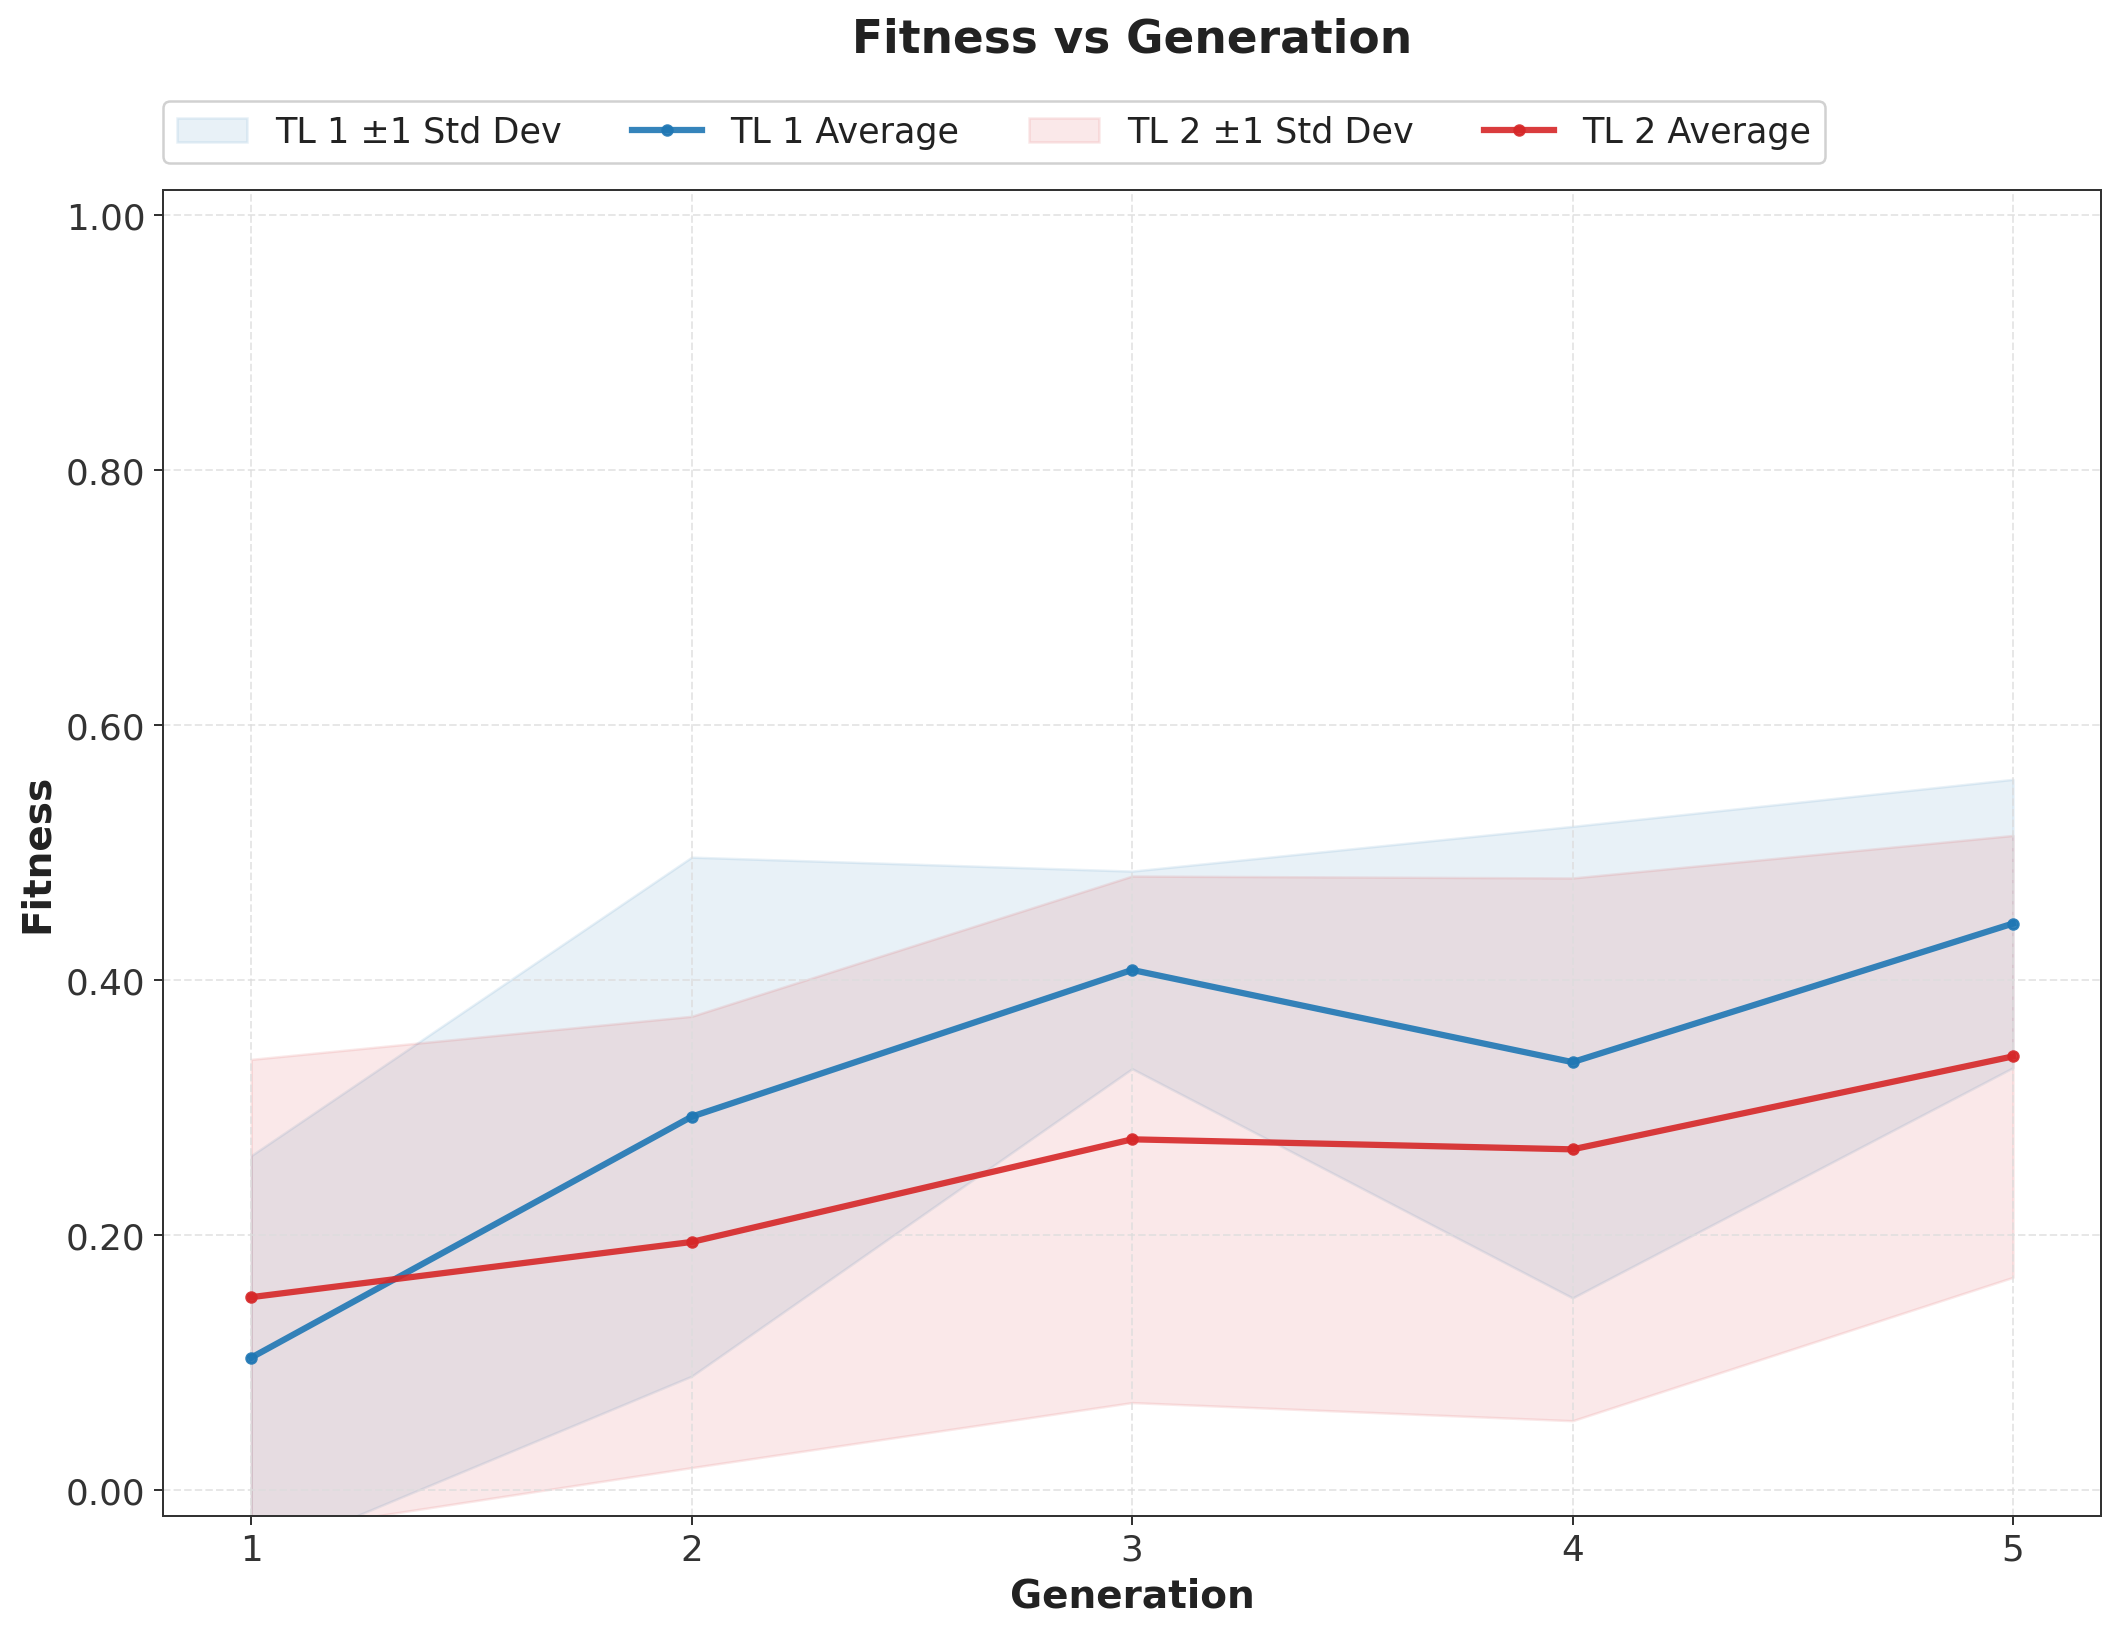
\includegraphics[width=0.45\textwidth]{../plots/plot_01_fitness_vs_gen.png}
\caption{Fitness vs Generation}
\label{fig:fitness_gen}
\end{figure}

As shown in Fig. \ref{fig:fitness_gen}, despite initial stochasticity and widespread failure in early generations, the Evolutionary Algorithm successfully and consistently drives the swarm toward highly optimized management policies across all independent runs. Notably, the fitness score converges and fluctuates around 0.7, with the absolute best elite policies peaking near 0.8, rather than climbing to a perfect 1.0. This plateau is an intentional feature of the multi-objective fitness function. SurvivalRate and SavingRate are actively competing factors: keeping more fish alive inherently requires spending more money on resources. The only theoretical way to achieve a perfect 1.0 fitness score would be to achieve 100\% survival while spending absolutely zero dollars. Because that is a biological and economic impossibility, the true target of the EA is to find the ``sweet spot'' (around 0.7) where biological welfare and financial efficiency are perfectly balanced, rather than chasing an impossible perfect score.


\begin{figure}[H]
\centering
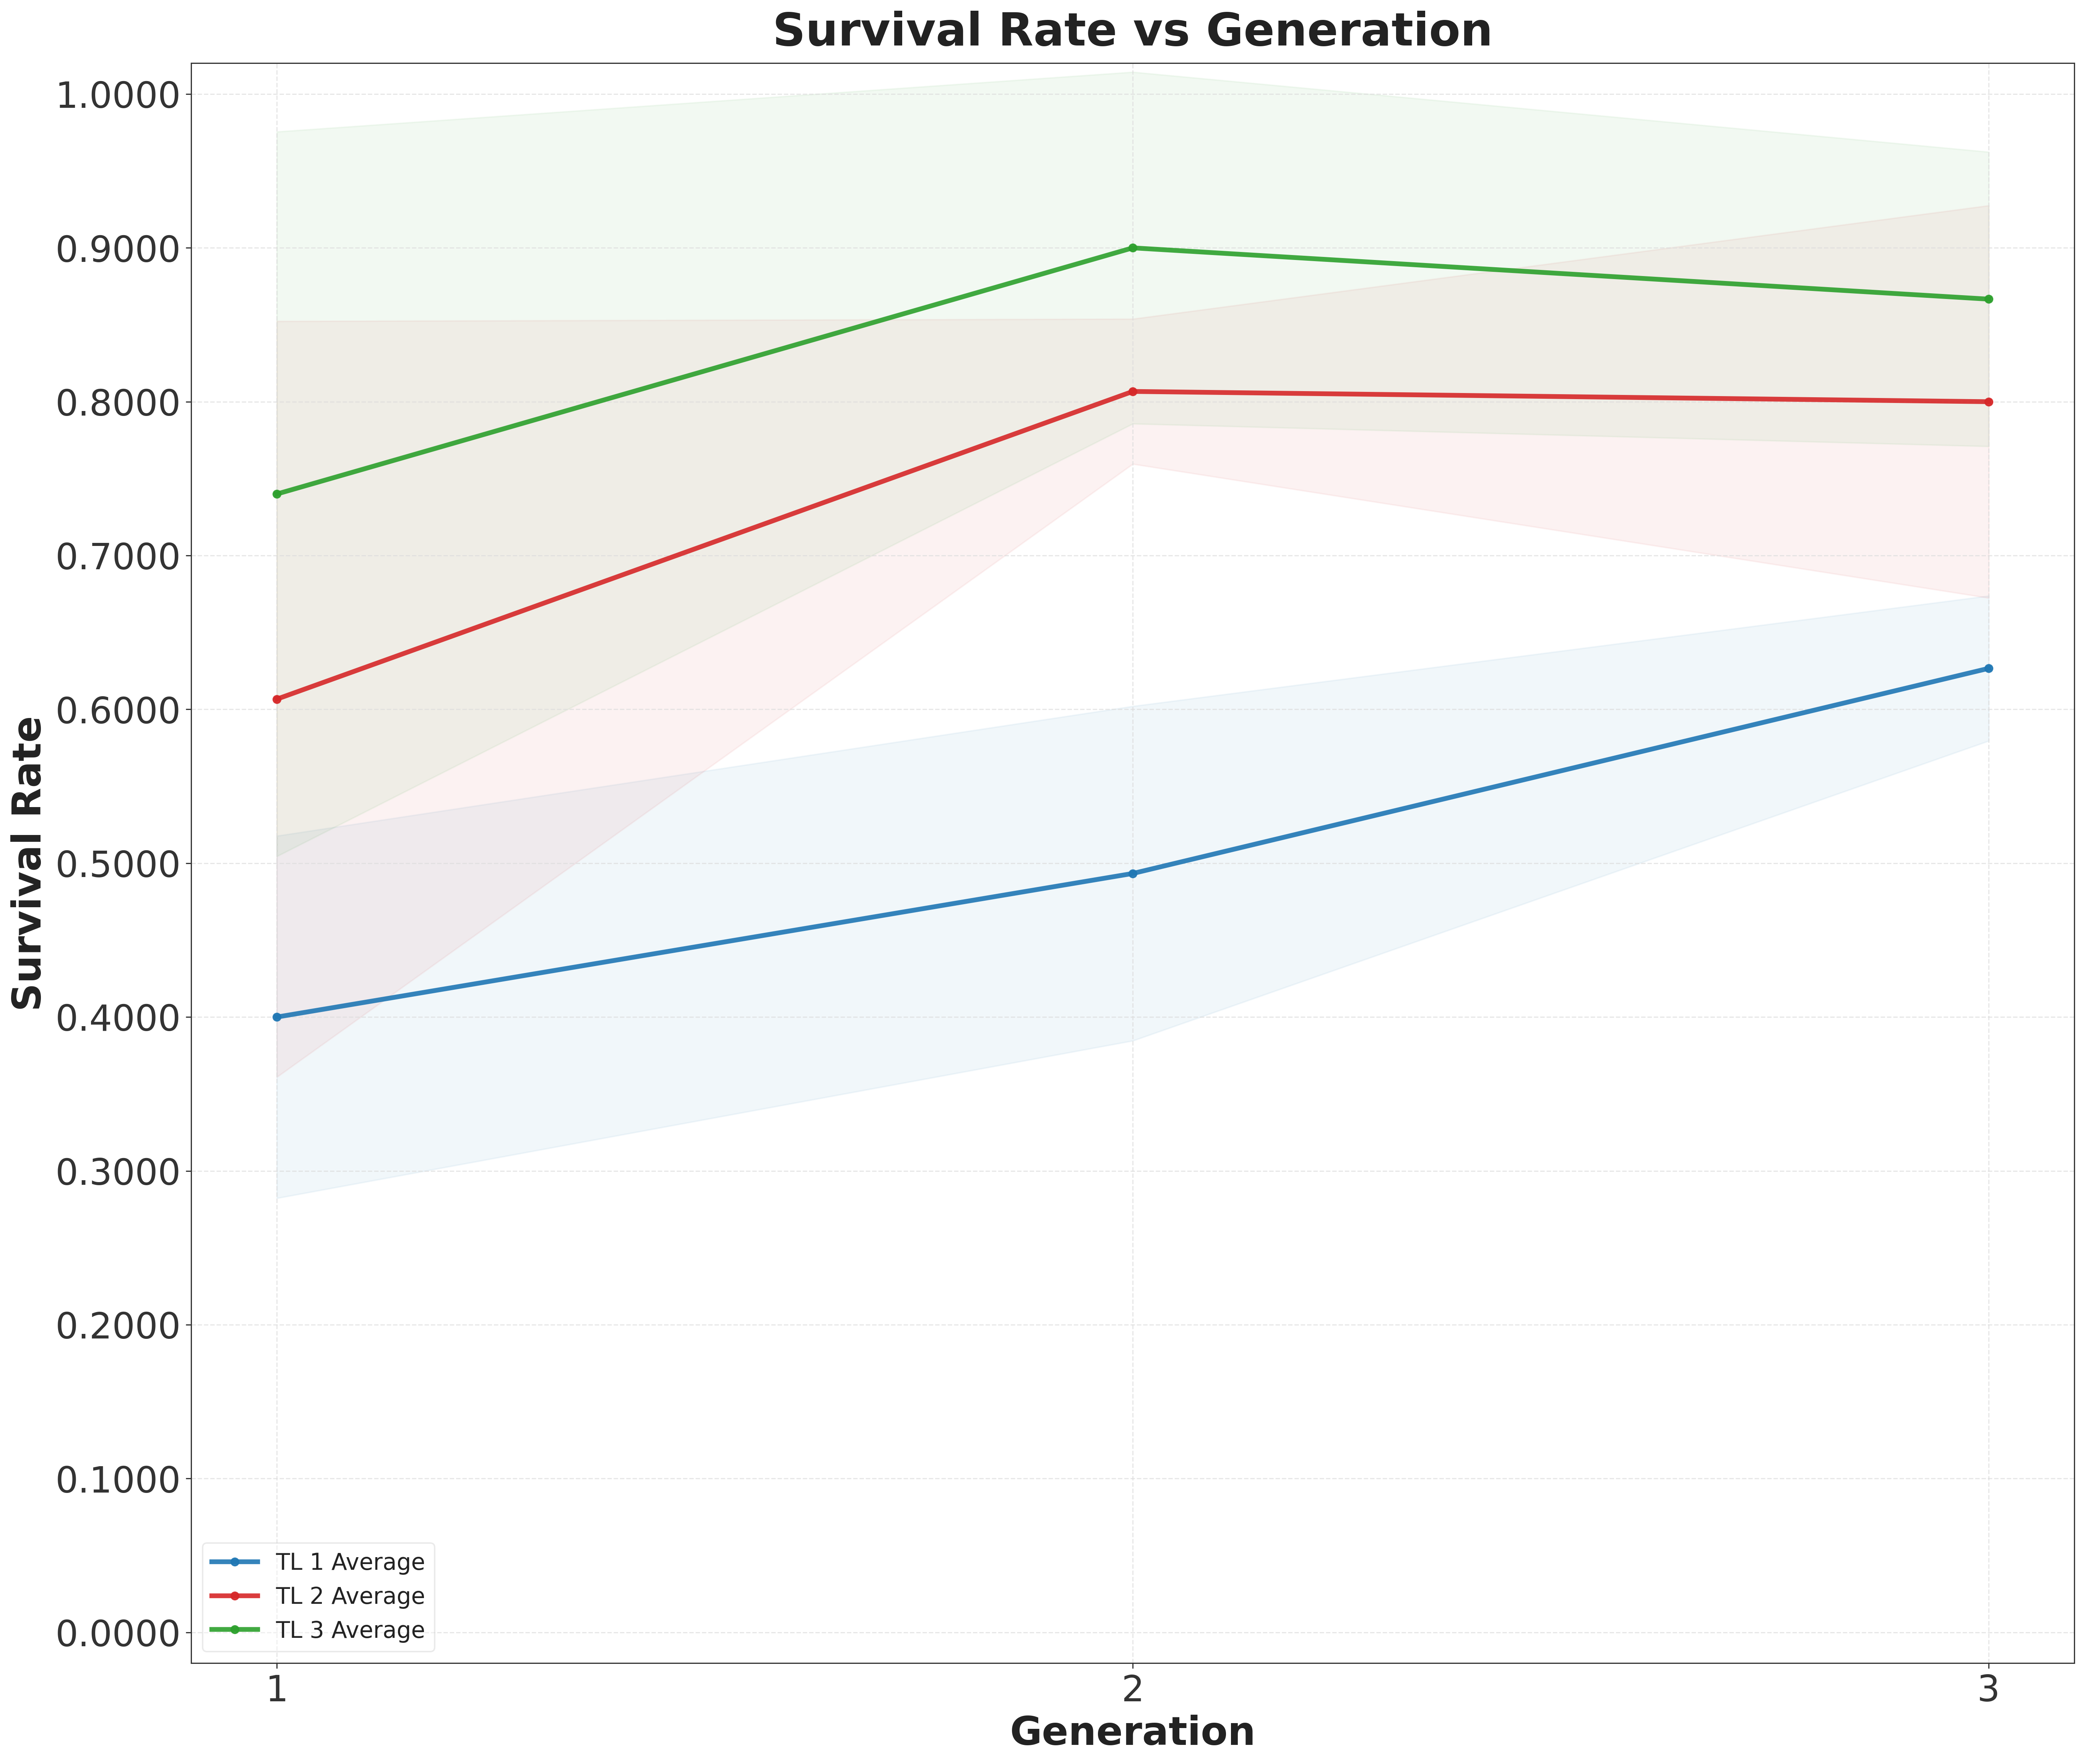
\includegraphics[width=0.45\textwidth]{../plots/plot_02_survival_rate_vs_gen.png}
\caption{Survival Rate vs Generation}
\label{fig:surv_gen}
\end{figure}

As depicted in Fig. \ref{fig:surv_gen}, the Survival Rate exhibits the most dramatic improvement among all metrics, climbing rapidly from an initial average near 0.2 up to a stable convergence around 0.8. Because Survival Rate is the most heavily weighted component of the fitness function ($0.55$), the EA aggressively optimizes for it first. The data indicates that in the chaotic, hazard-rich virtual pond, early random policies fail disastrously, leading to massive population wipeouts. However, within just 5 to 7 generations, the algorithm successfully discovers and propagates foundational policies that keep the vast majority of the swarm alive through the full 30-day cycle.


\begin{figure}[H]
\centering
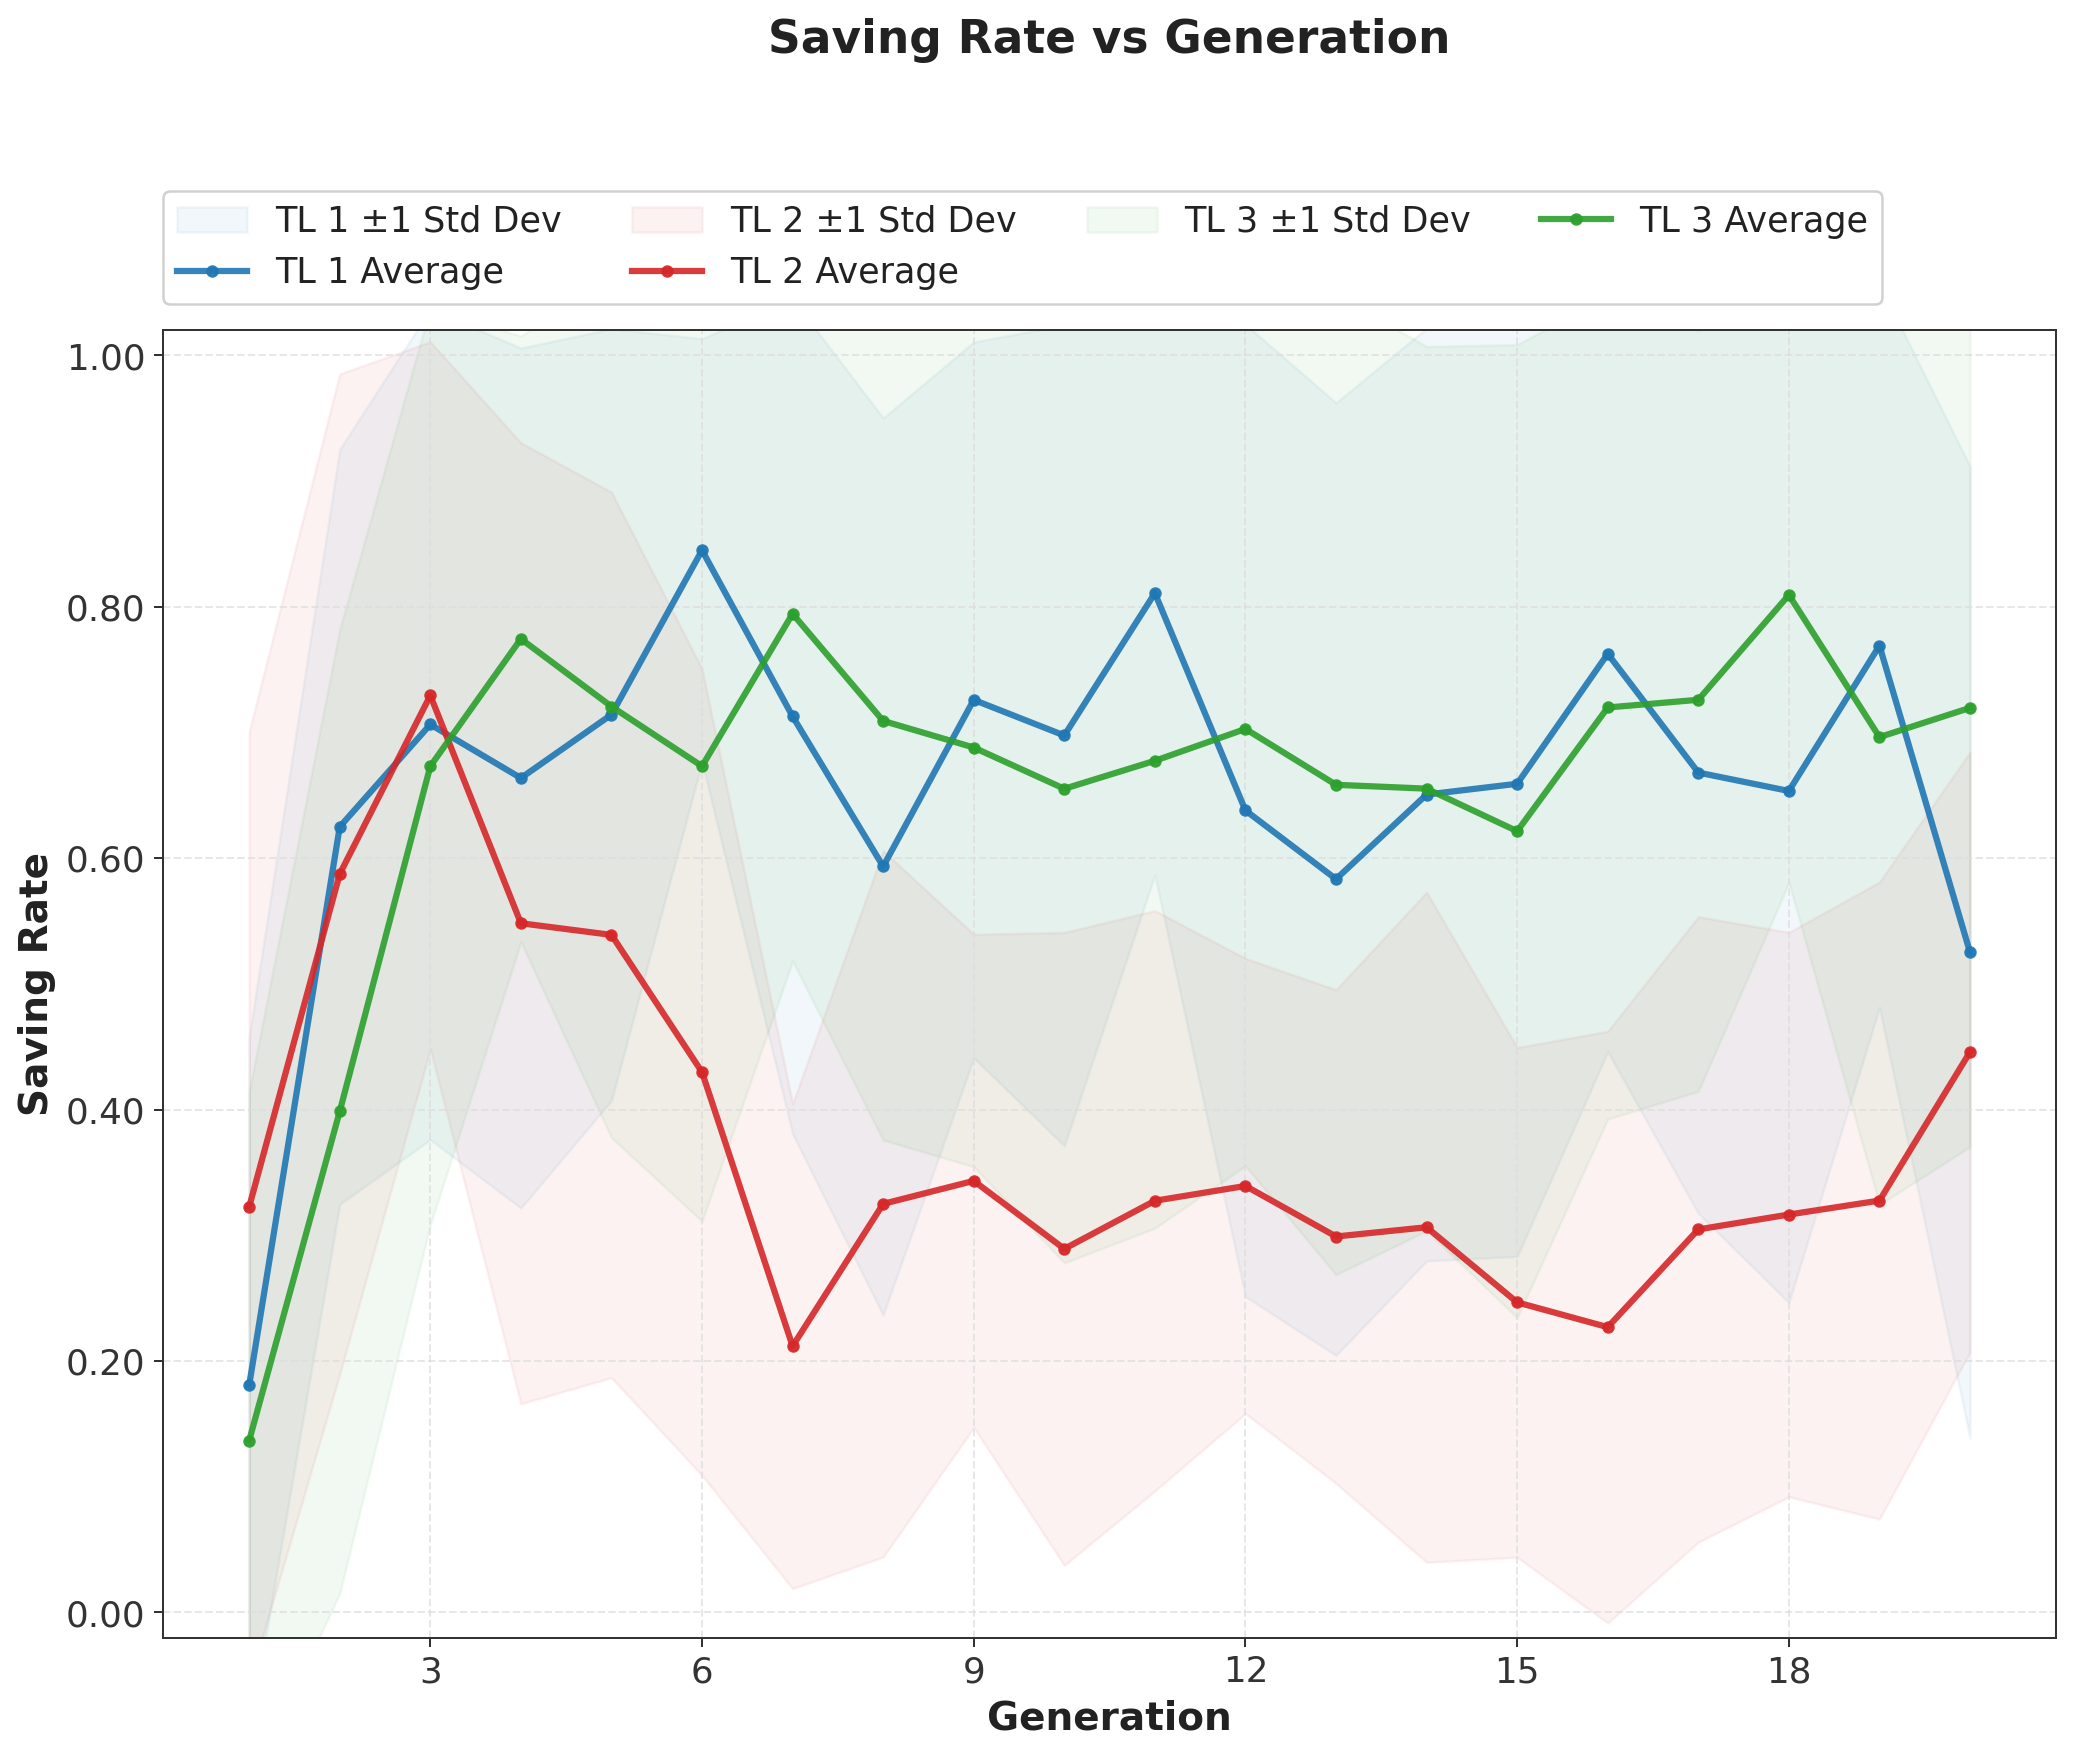
\includegraphics[width=0.45\textwidth]{../plots/plot_03_saving_rate_vs_gen.png}
\caption{Saving Rate vs Generation}
\label{fig:saving_gen}
\end{figure}

Fig. \ref{fig:saving_gen} illustrates the evolutionary trajectory of the Saving Rate. Unlike the rapid, unidirectional climb of the Survival Rate, the Saving Rate experiences a slight initial dip before slowly recovering and stabilizing around 0.6. This curve perfectly captures the ``cost of learning.'' In early generations, the EA attempts to maximize survival by over-allocating resources---dumping excessive food and oxygen into the pond to prevent fish death. Once the swarm achieves a stable survival baseline, the algorithm begins to incrementally refine the policies, stripping away excess resource expenditures to optimize the secondary Saving Rate metric without triggering starvation or hypoxia.


\begin{figure}[H]
\centering
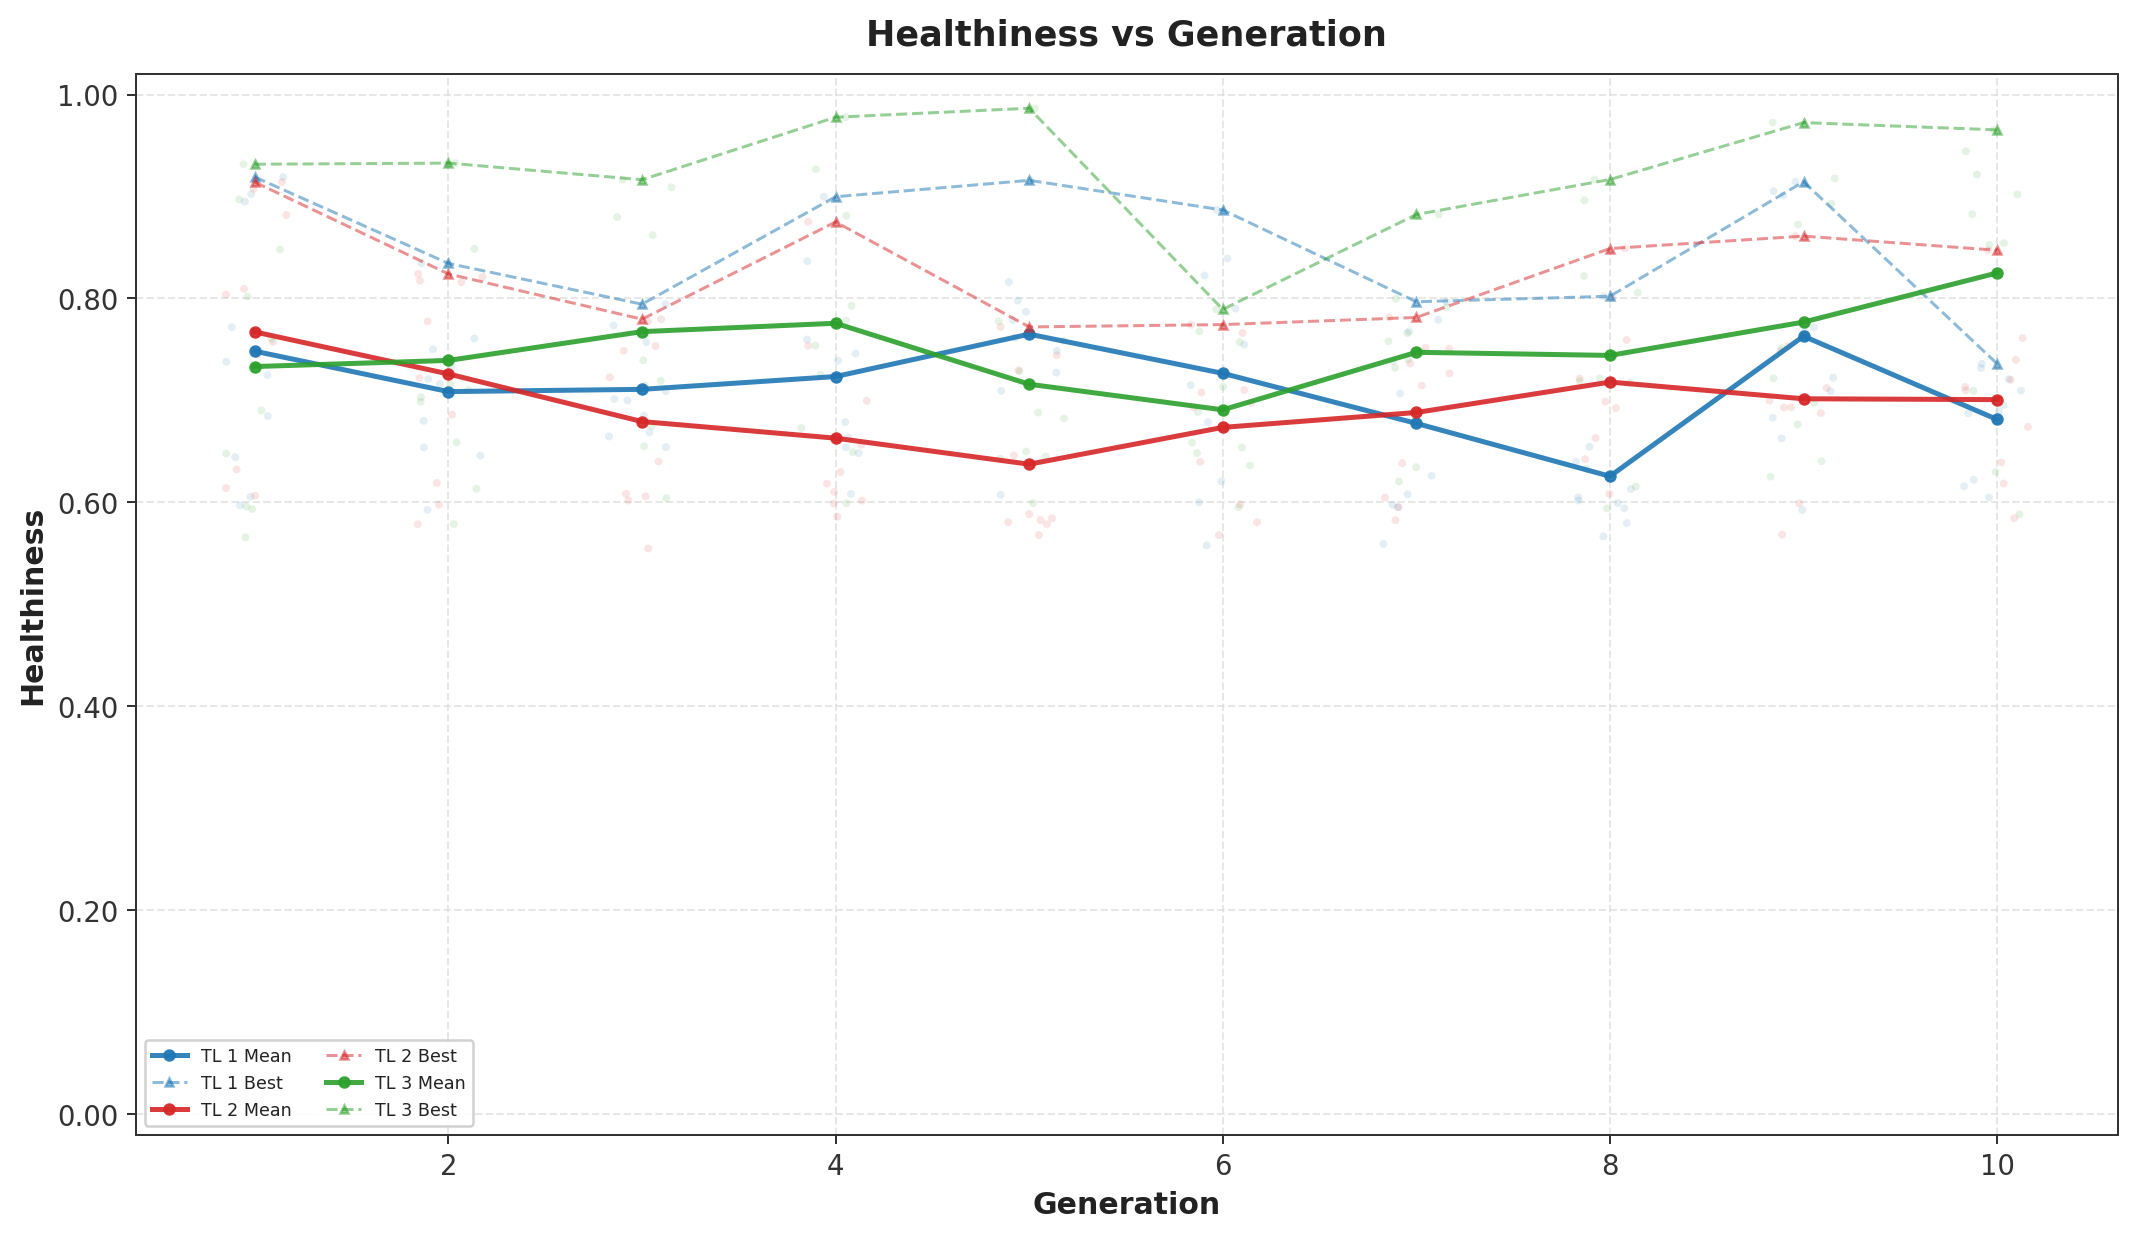
\includegraphics[width=0.45\textwidth]{../plots/plot_04_healthiness_vs_gen.png}
\caption{Healthiness vs Generation}
\label{fig:health_gen}
\end{figure}

Fig. \ref{fig:health_gen} maps the Healthiness metric across the generations. This metric converges to a relatively high baseline (between 0.7 and 0.8) very quickly. Because Healthiness is intrinsically tied to survival---a fish cannot survive the 30-day simulation if its health drops to zero---any policy that manages to achieve a high Survival Rate naturally results in a surviving population with an acceptable health baseline. Since it carries the lowest weight ($0.12$) in the fitness function, it acts strictly as a fine-tuning tie-breaker in later generations, ensuring that surviving fish are not left in a perpetually starved or diseased state.


\begin{figure}[H]
\centering
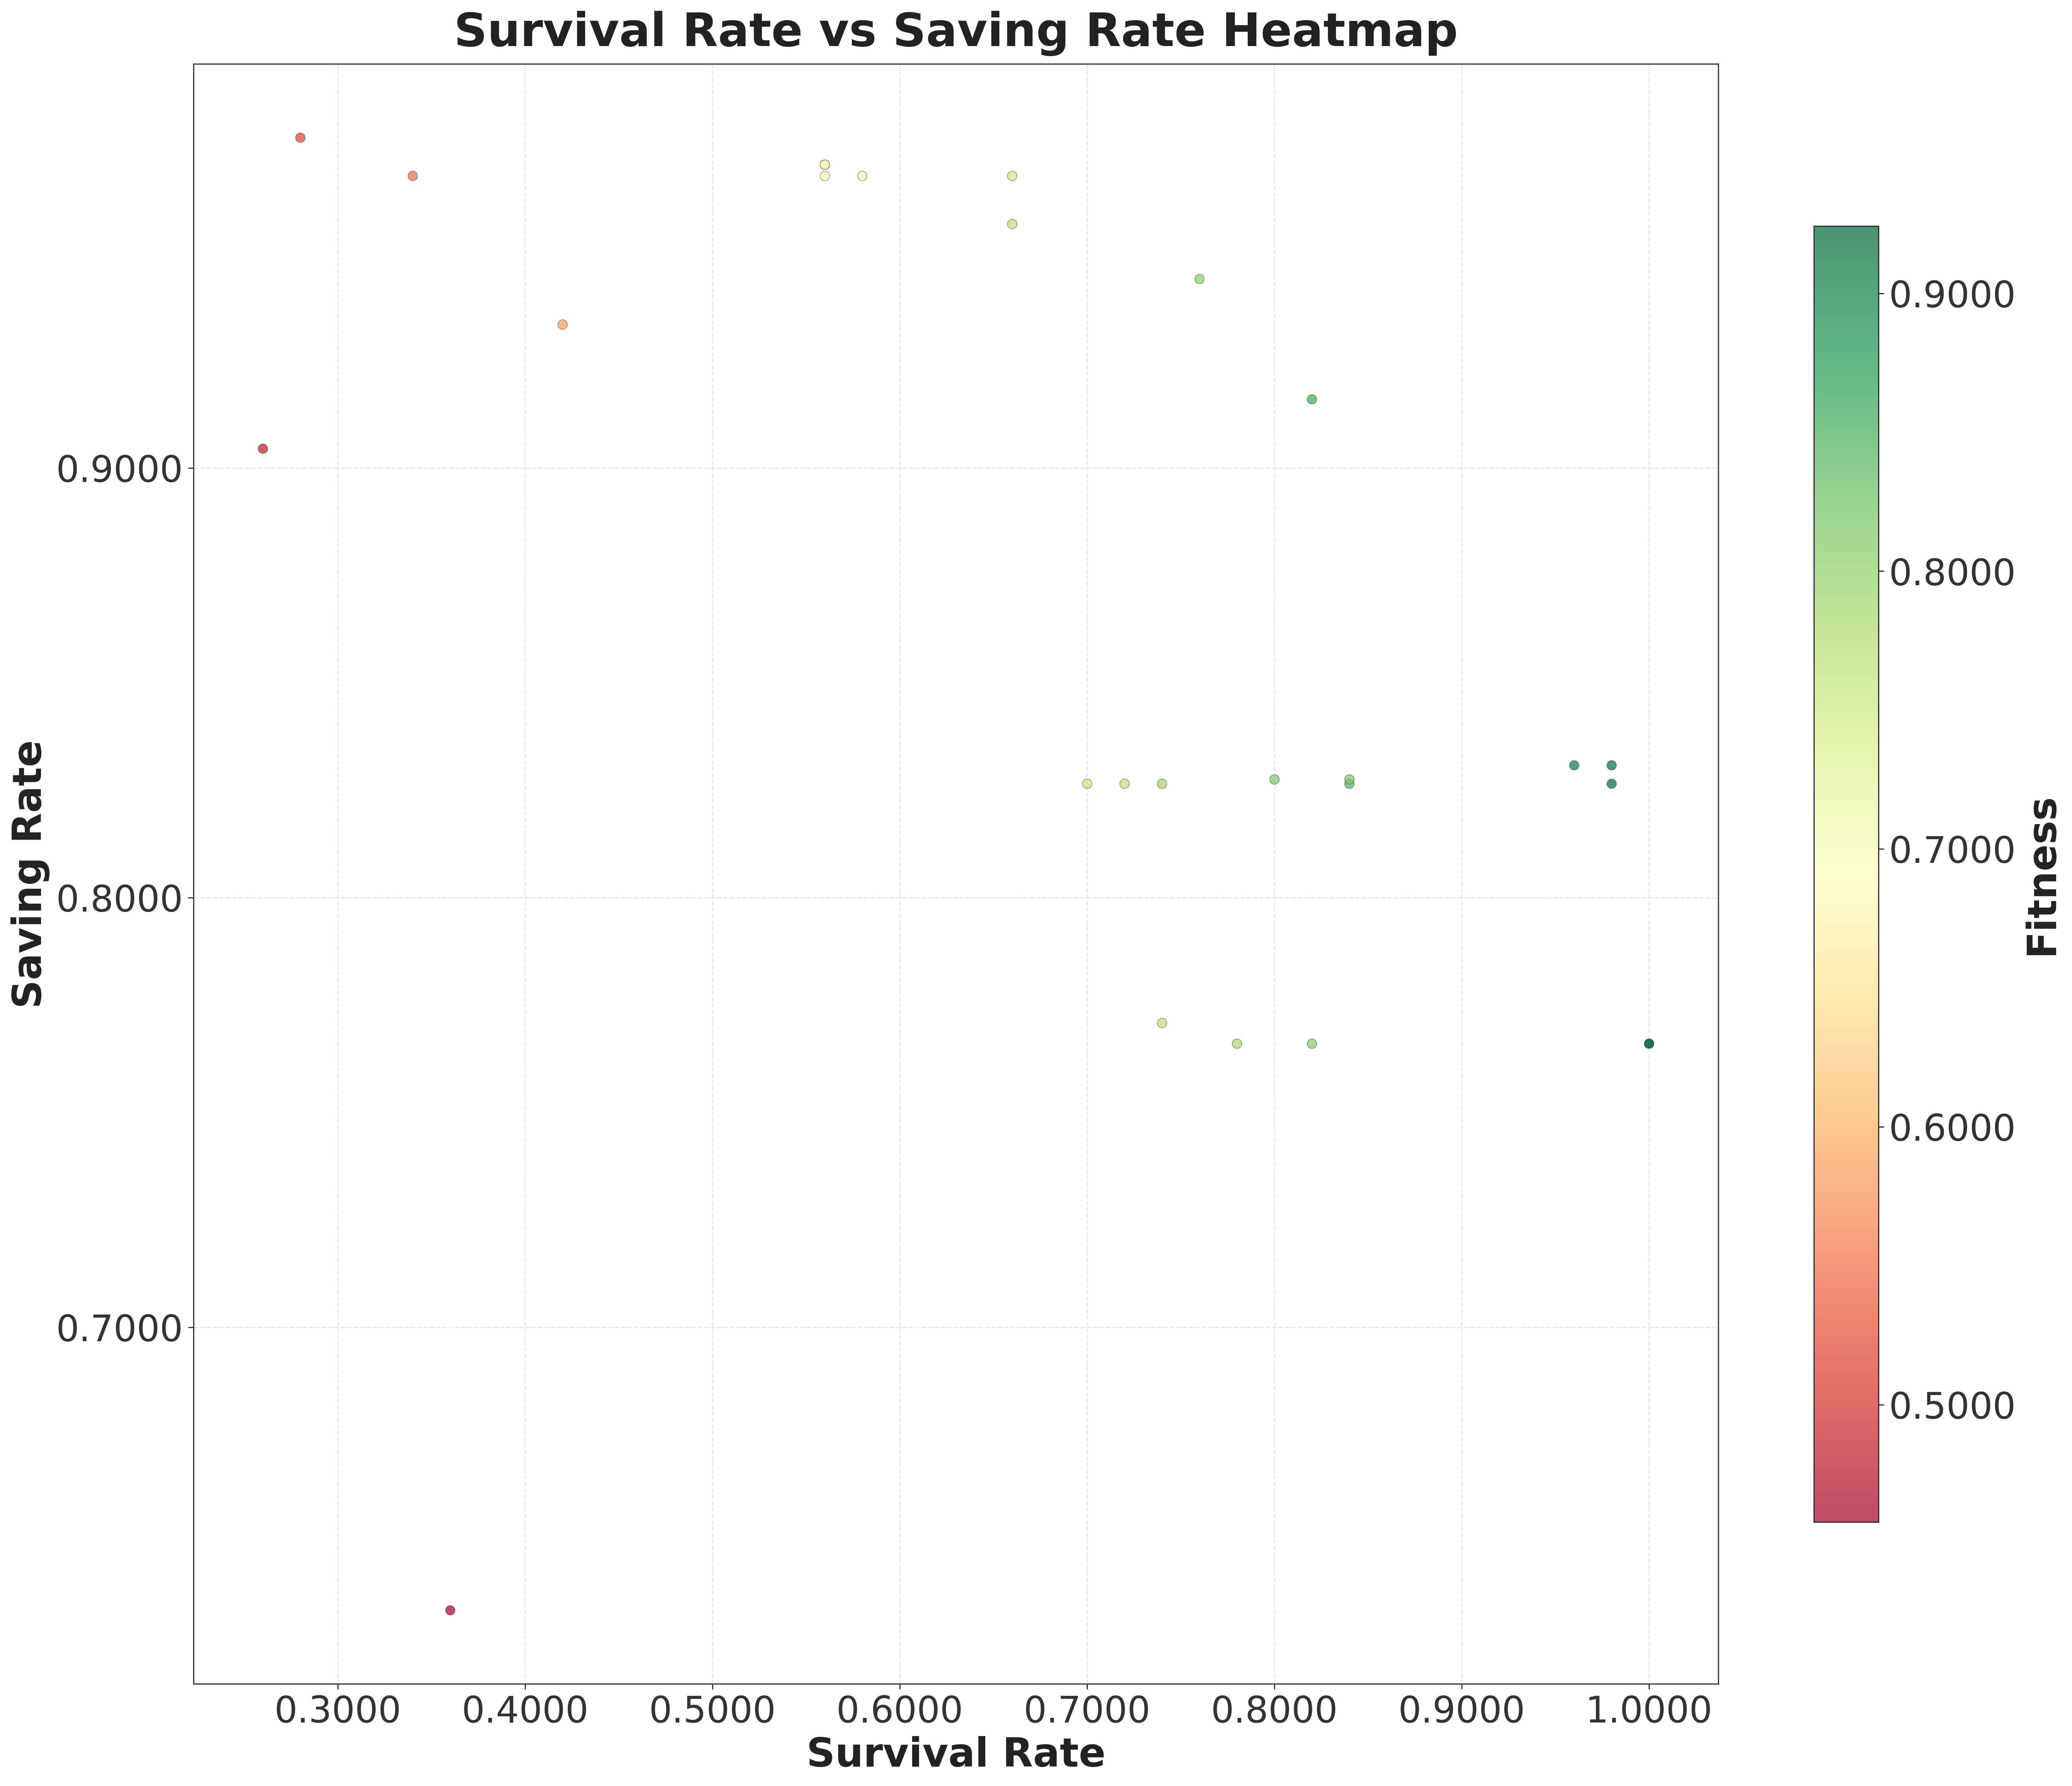
\includegraphics[width=0.45\textwidth]{../plots/plot_05_survival_rate_vs_saving_rate_heatmap.png}
\caption{Survival Rate vs Saving Rate Heatmap}
\label{fig:heat_surv_saving}
\end{figure}

The heatmap in Fig. \ref{fig:heat_surv_saving} reveals the dense clustering of evaluated policies regarding Survival versus Savings. The intense concentration in the upper-right quadrant visually confirms the EA's success in finding optimal ``sweet spots.'' Notably, there is an absolute void in the extreme top-right corner (1.0 Survival, 1.0 Savings), mathematically proving that zero-cost survival is impossible in this environment. The distinct clusters also demonstrate that the algorithm frequently encounters a sharp Pareto frontier: to push survival from 80\% to 90\%, the policy must disproportionately sacrifice budget. Furthermore, the red dots scattered in the lower-left region of the plot reveal an interesting phenomenon: excessive spending can actually backfire. If the budget is heavily drained by dumping too much food and probiotics into the pond, the unconsumed leftovers decay into pollutants. These pollutants then transform into environmental hazards that harm the fish, paradoxically leading to a lower survival rate despite the high resource expenditure.


\begin{figure}[H]
\centering
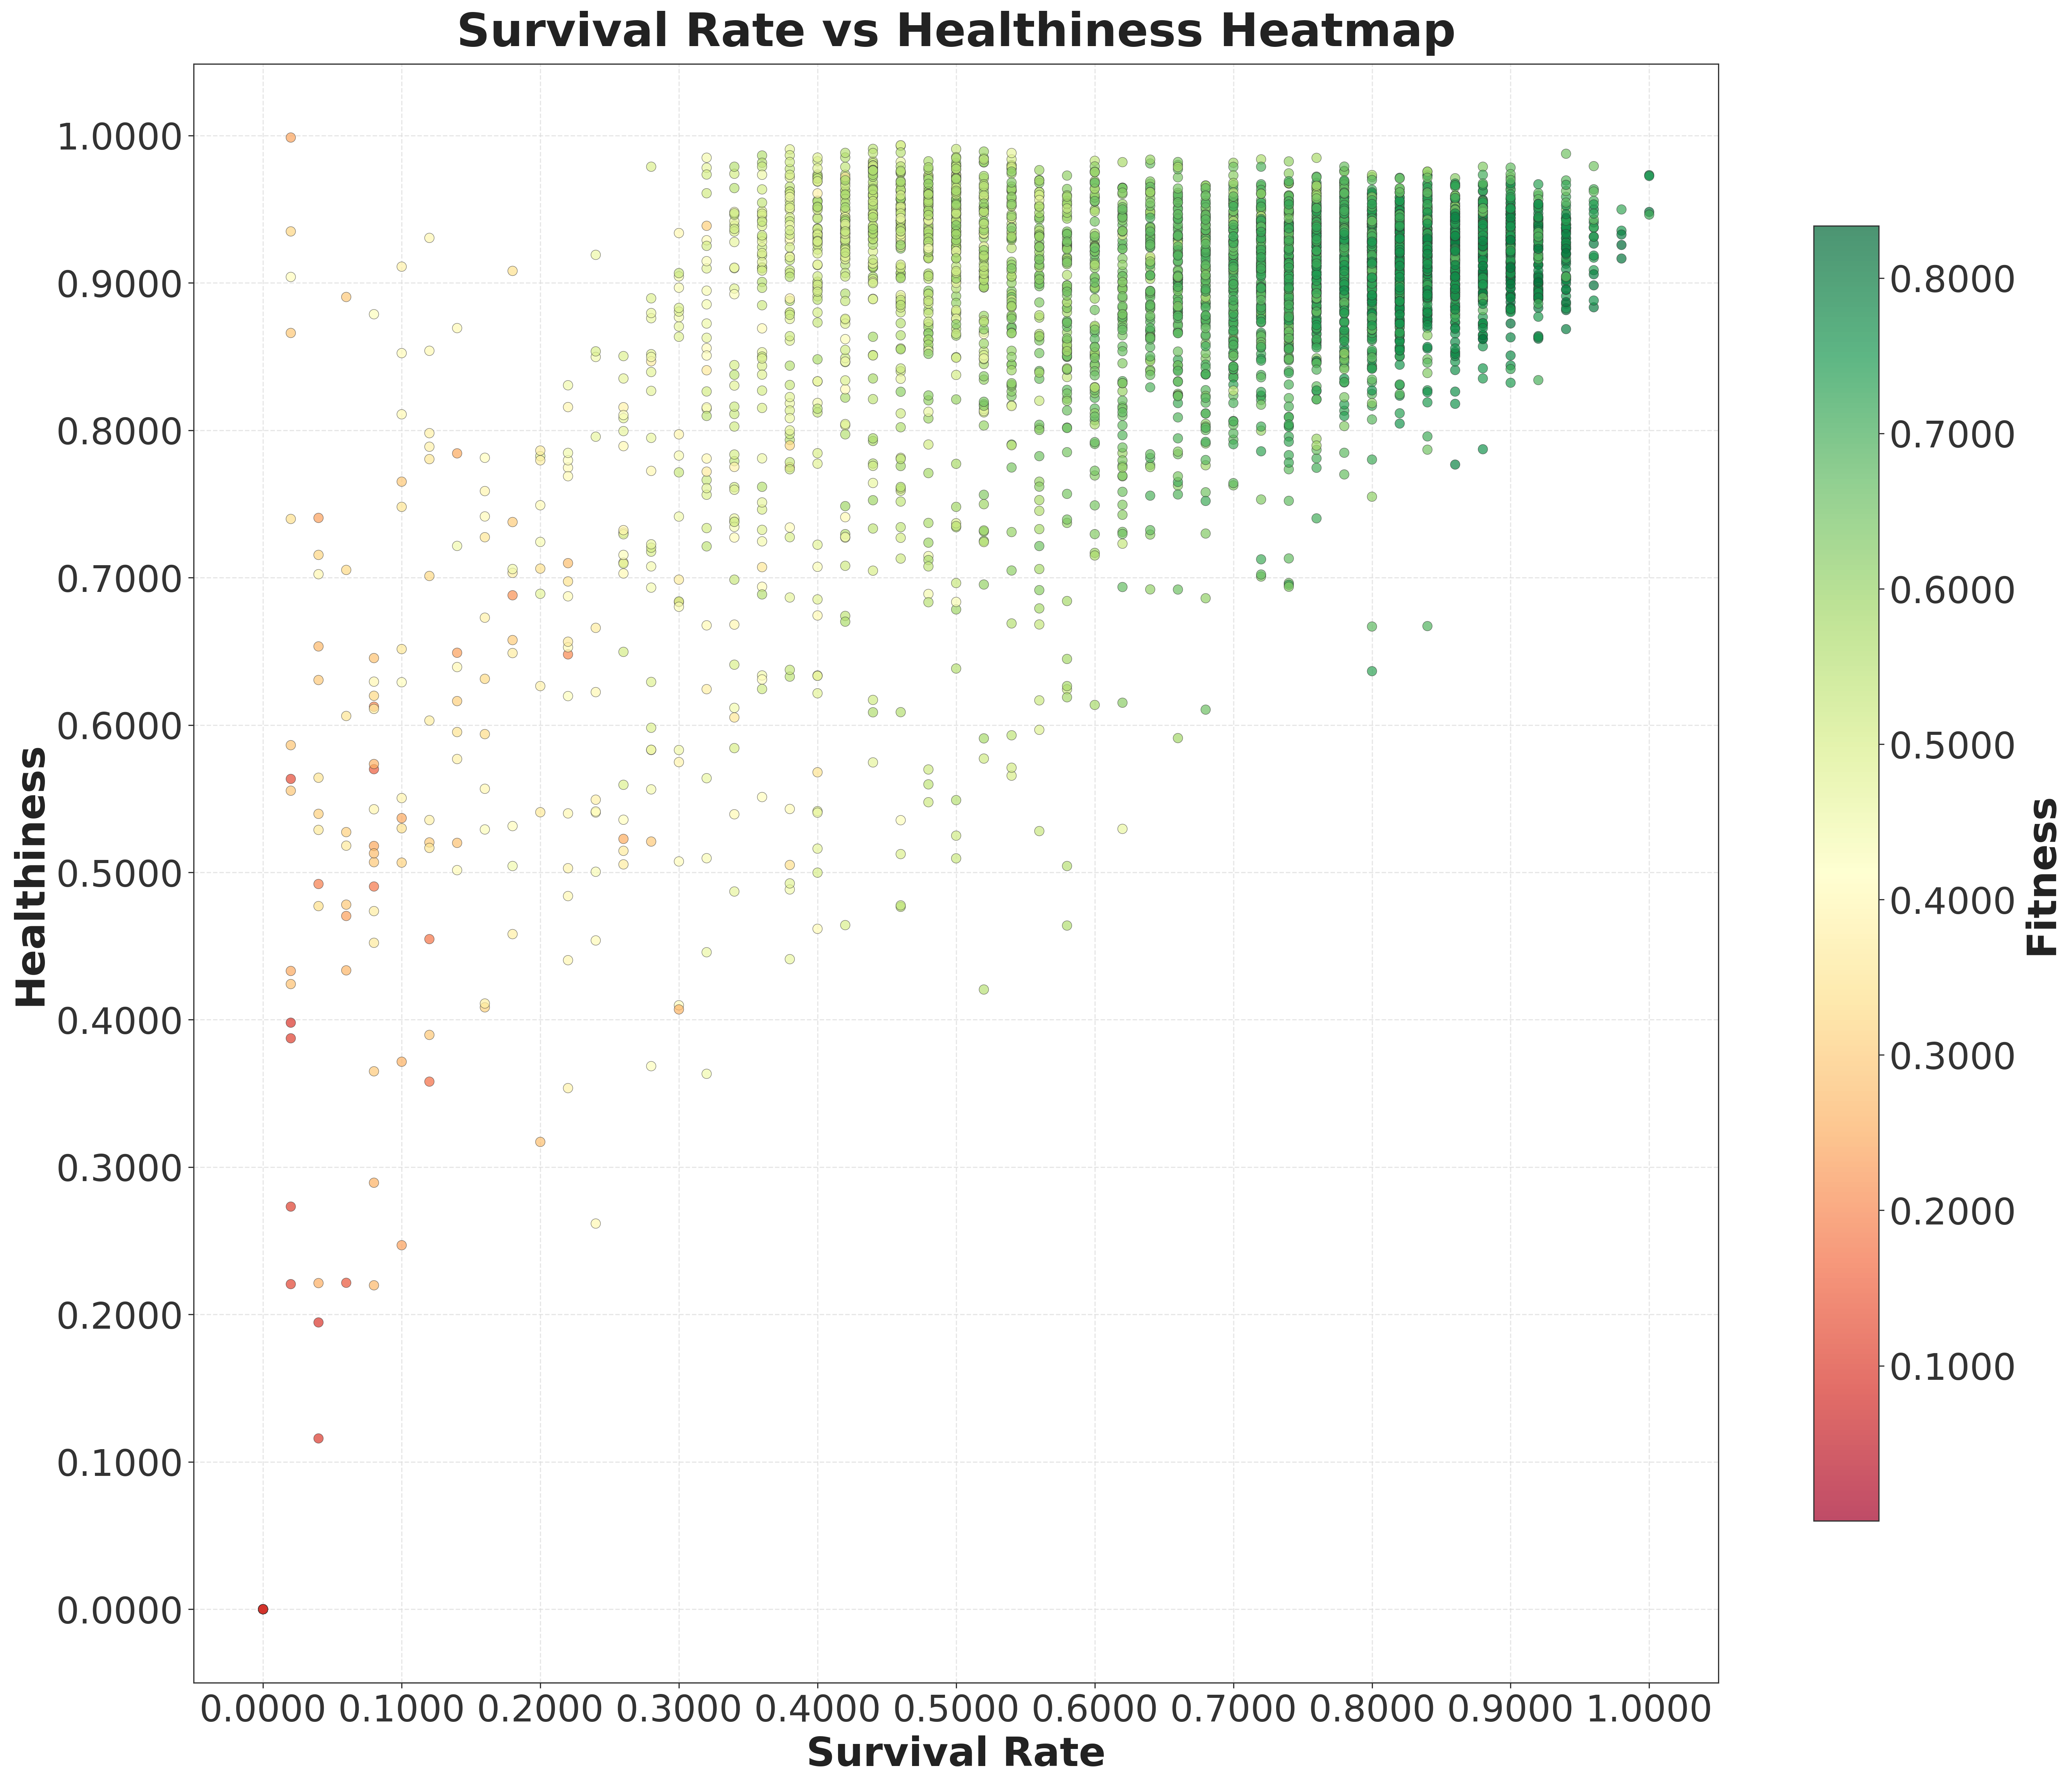
\includegraphics[width=0.45\textwidth]{../plots/plot_06_survival_rate_vs_healthiness_heatmap.png}
\caption{Survival Rate vs Healthiness Heatmap}
\label{fig:heat_surv_health}
\end{figure}

Fig. \ref{fig:heat_surv_health} illustrates the strong positive correlation between Survival Rate and Healthiness. The dense, diagonal clustering indicates that these two metrics are highly synergistic rather than strictly competitive. Policies that successfully mitigate environmental hazards (like NH3 and parasites) and provide adequate nutrition naturally result in both higher survival numbers and higher average internal physiological scores for those survivors.


\begin{figure}[H]
\centering
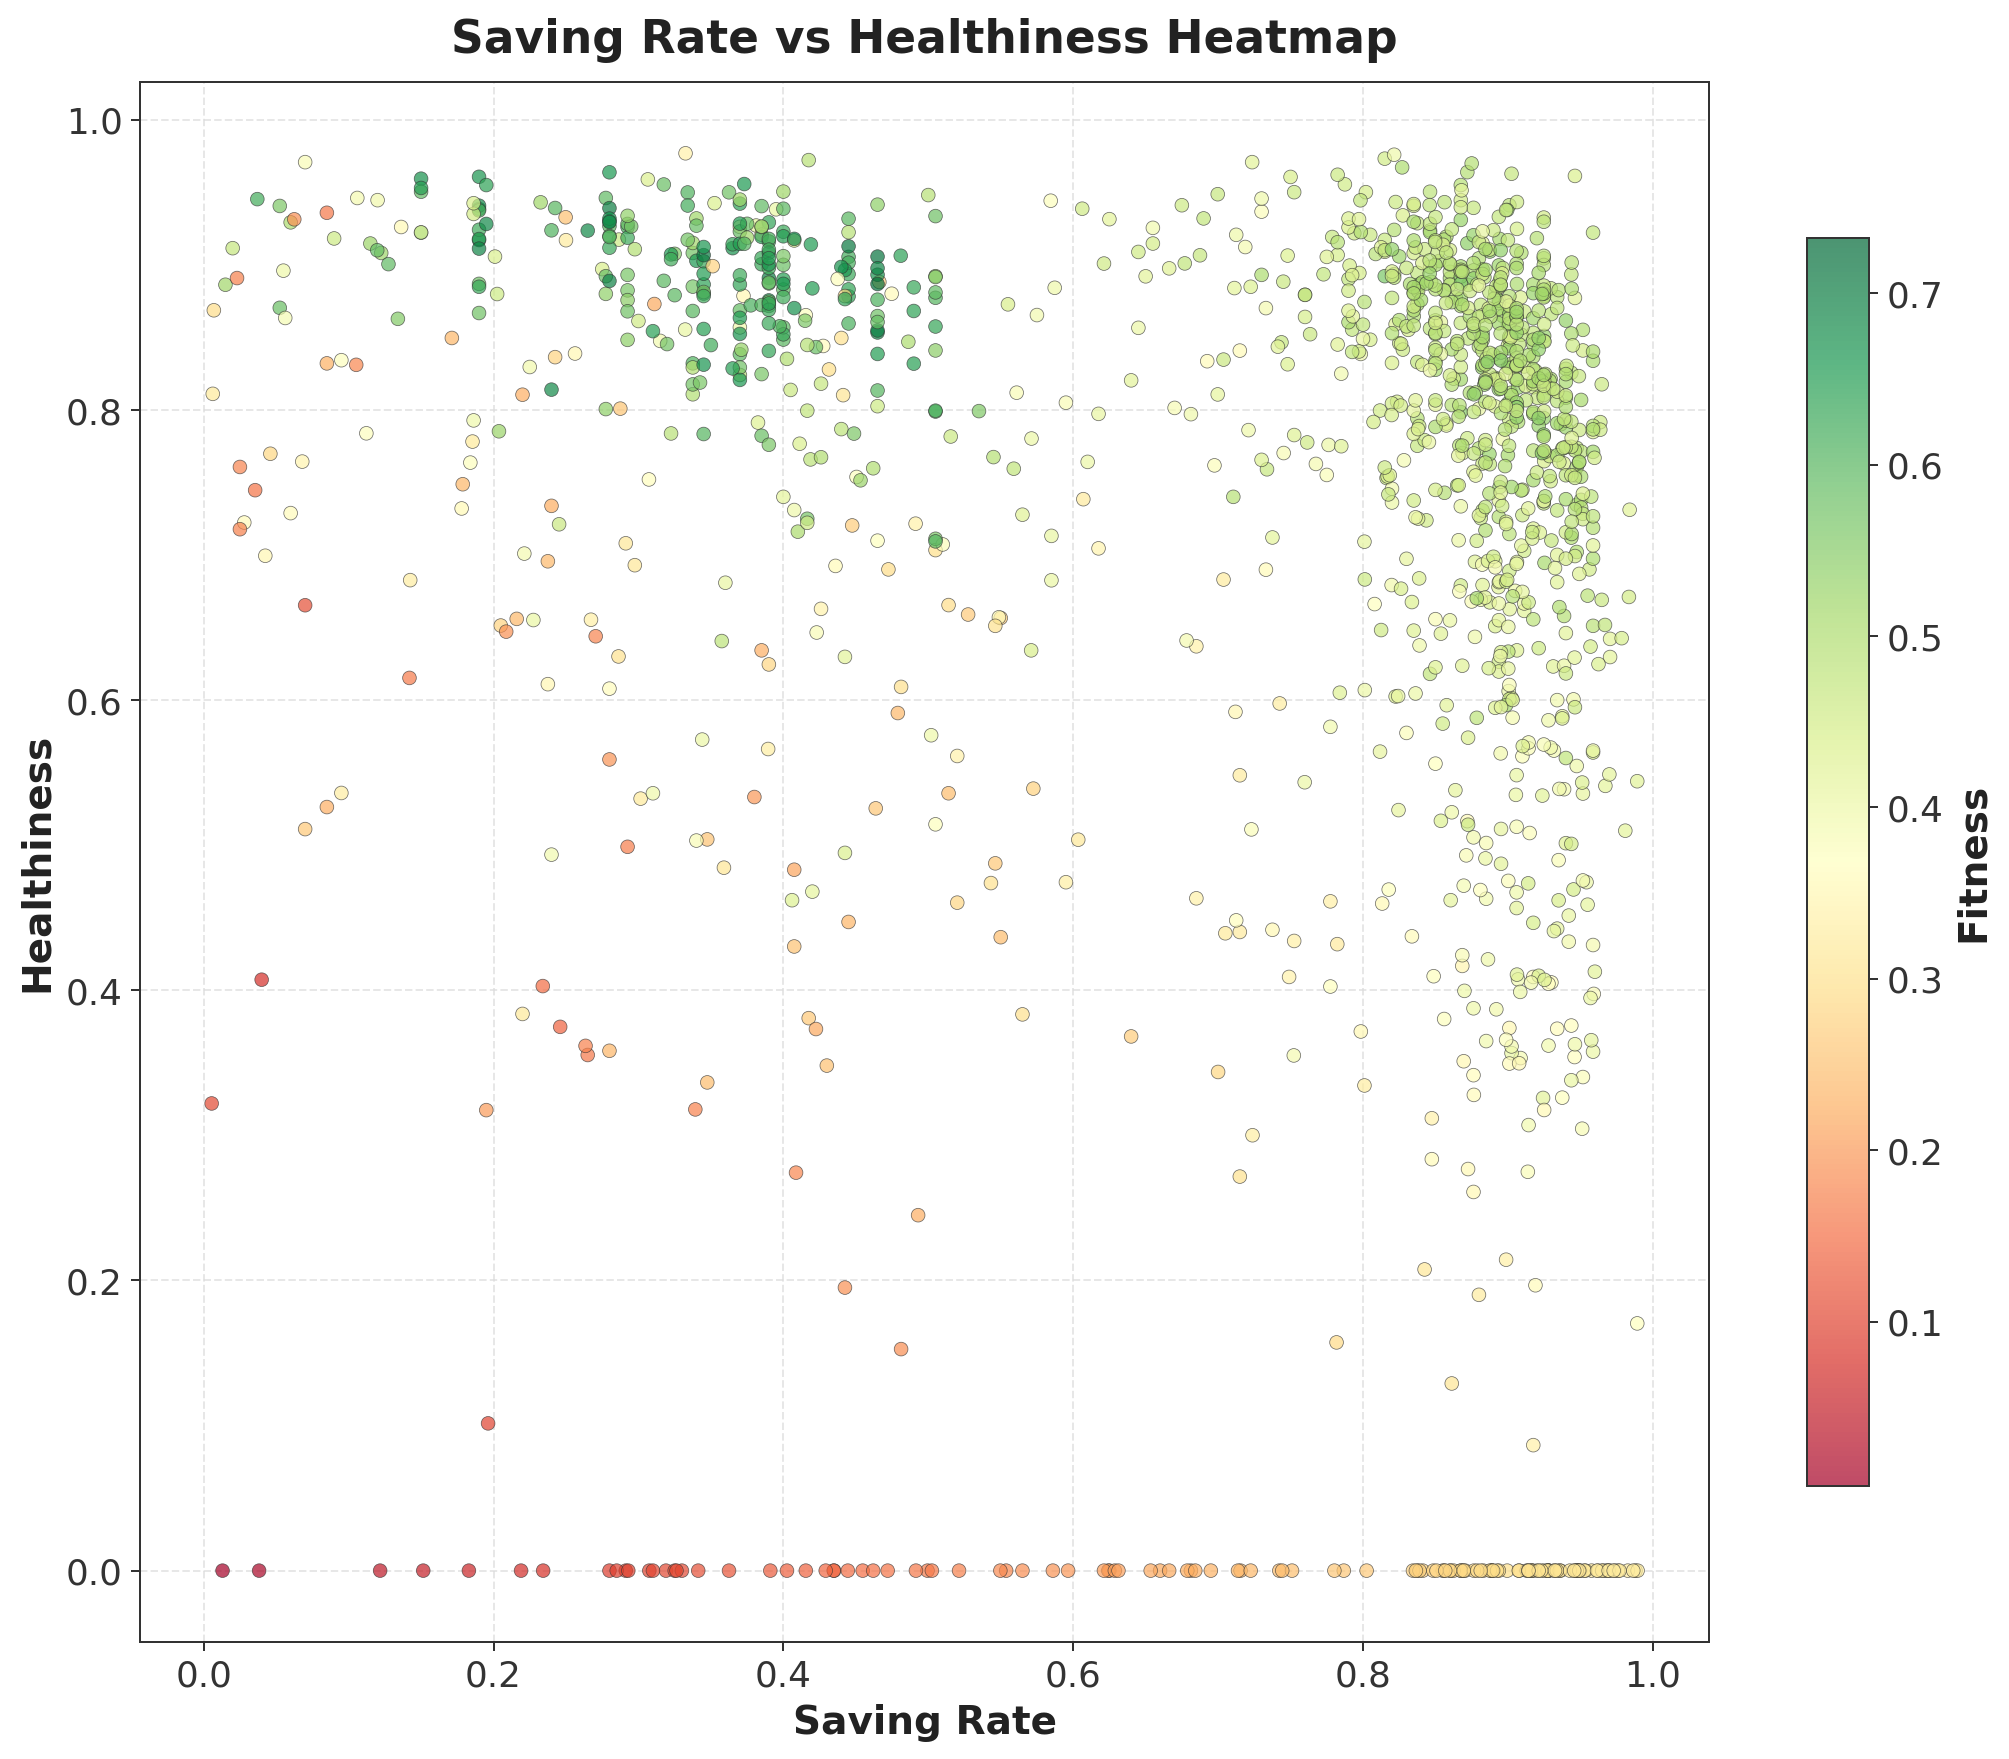
\includegraphics[width=0.45\textwidth]{../plots/plot_07_saving_rate_vs_healthiness_heatmap.png}
\caption{Saving Rate vs Healthiness Heatmap}
\label{fig:heat_saving_health}
\end{figure}

Finally, Fig. \ref{fig:heat_saving_health} maps Saving Rate against Healthiness. This plot shows a much wider dispersion compared to the other heatmaps, indicating a complex, non-linear relationship. While it is possible to achieve high health and decent savings (the hot spot in the upper-right center), there is a significant spread. This spread suggests that poorly timed resource drops can waste the budget without improving fish health, while highly optimized, precisely timed drops (developed in later generations) can maintain top-tier health without exhausting the budget. Because Healthiness is intimately linked with the Survival Rate, this non-linear relationship also reflects the overspending backfire effect observed earlier: excessively dumping resources drains the budget and creates water-degrading pollutants. These resulting hazards aggressively attack the immune systems of the fish, causing overall health to plummet even when financial resources were abundantly spent.




As shown in Fig. \ref{fig:geno_food}, the EA's optimization of the food quantity gene reveals that it does not converge to a single small value, but rather fluctuates continuously within the range of 5 to 10 pellets. This flexible buffer exists because the swarm's caloric needs constantly vary due to the highly stochastic environment; keeping the quantity slightly elevated and fluctuating ensures that the fish are not accidentally starved into intracohort cannibalism during highly active evasion periods. Conversely, the food drop interval tightly converges down to a controlled cycle of approximately 5 to 6 hours. Furthermore, the bar patterns in the plot visualize the spatial Location gene, where solid bars represent Center drops and hatched bars represent Random drops. For food, the location firmly converges toward the hatched Random distribution. This behavior highlights the EA's understanding of the environment's physics: dropping resources exclusively in the center fails to reach lonely, isolated fish and concentrates decaying waste into a single, highly dangerous point of pollution. By spreading the drops randomly and feeding every 5-6 hours, the policy ensures the whole swarm is safely fed while mitigating localized ammonia spikes.

Fig. \ref{fig:geno_prob} tracks the evolution of probiotic treatments. Because probiotics are incredibly expensive (\$0.50 per pellet), the EA must be highly conservative. The convergence plot reveals that the optimal strategy is to apply probiotics very sparsely—typically 1 to 2 pellets every 48 to 72 hours. Unlike the Food genotype, the bar patterns (solid for Center, hatched for Random) indicate that the Location gene never truly converges, instead fluctuating continuously between the two states. This fluctuation suggests that the specific drop location of probiotics does not significantly impact survival; because the quantity is so incredibly small relative to the total number of objects and the sheer volume of the pond, the exact placement is mathematically trivial. Ultimately, the EA learned to use probiotics not as a daily dietary supplement, but rather as a calculated, preventative ``bump'' to the fishes' immunity, keeping the swarm robust against the occasional random disease spawn without crippling the Saving Rate.

The Oxygen Genotype Convergence in Fig. \ref{fig:geno_oxy} reveals a fascinating biological optimization heavily driven by economic constraints. The EA firmly converges the pumping duration to exactly 1 hour. Because Oxygen is the most expensive resource (\$1.50 per hour), the algorithm aggressively suppresses duration to maximize the Saving Rate. However, the pumping interval does not strictly converge, instead fluctuating in a wide range between 12 and 24 hours. This wide variance indicates that the PSO-driven fish are remarkably resilient to localized hypoxia; they can survive extended periods without fresh oxygen injection by actively swimming away from hazardous zones or shifting towards the surface. Finally, the bar patterns demonstrate a beautiful convergence of the Location gene toward the hatched Random distribution. Because environmental hazards like NH3 bubbles are not strictly stationary but instead slowly moving through the pond, they create unpredictable, moving ``dead zones.'' Randomly placing the oxygen source ensures that the fish are not forced to repeatedly swim into these potentially hazardous central clusters just to breathe, significantly improving overall survival while minimizing redundant pumping costs.

Fig. \ref{fig:pop_dist} categorizes the outcomes of all evaluated policies into four possible statuses: OK (solid bars, indicating the policy finished the 30-day simulation within budget with at least one survivor), ALL-DEAD (all fish died before day 30), OVER-BUDGET (policy spent more than \$500 during the simulation), and REJECT. The Reject status is a pre-calculated early termination that immediately discards a genotype if its hard-coded parameters mathematically exceed the maximum budget, saving significant computational cost by skipping the simulation entirely. Interestingly, there are zero Reject cases observed, meaning all generated policies were at least theoretically viable before execution. In the early generations, the chart is dominated by OVER-BUDGET and ALL-DEAD failures as random policies either aggressively overspend or starve the fish. The ultimate target is to maximize the solid OK sections. By Generation 20, the distribution shifts dramatically, with over 80\% of the policies successfully completing the simulation in the OK status, visually confirming the robustness of the genetic convergence across all timelines.

The Champion Comparison plot (Fig. \ref{fig:champ_comp}) extracts the single best elite policy from the final generation of each of the 10 timelines. The data reveals a significant variance among these champions: Timeline 10 produced the absolute best policy with a peak Fitness of 0.8158, while Timeline 3 produced the worst champion at 0.7498, against an overall champion average of approximately 0.7885. A deeper look into the secondary metrics reveals fascinating contradictions: the lowest-scoring champion (Timeline 3) actually achieved the highest Saving Rate of the entire group. Conversely, Timeline 9 recorded the lowest Saving Rate but still managed to secure an average overall Fitness score. This confirms the highly complex, non-linear correlation between Fitness and Saving Rate, and strongly implies that the noisy, stochastic nature of the environmental setup means ``luck'' remains a significant factor in a policy's final evaluation. Because of this inherent environmental noise, it is highly probable that Timeline 10's peak score of 0.8158 was bolstered by a more forgiving randomized hazard setup, and its specific genotype might not consistently reproduce that exact peak across multiple random seeds. Therefore, rather than declaring a single definitive winner based on environmental luck, the robust champion average of approximately 0.7885 represents the true, realistic ``sweet spot'' of fitness that a highly optimized management policy can reliably achieve in this chaotic system.

Table \ref{tab:champ_tl10} details the specific performance metrics and decoded genotype of this TL-10 Champion. The policy achieved a remarkable 94\% Survival Rate (47 out of 50 fish survived) while spending only \$208.50 of the \$500 budget. Analyzing its genotype reveals a fascinating emergent strategy regarding resource allocation. While its Food and Oxygen genes align perfectly with the overall convergence trends (frequent random feeding to prevent cannibalism, and sparse, randomly located oxygen pumping to maximize savings), its Probiotic gene is striking: the quantity is exactly 0 pellets. The EA completely abandoned the use of incredibly expensive probiotics. Instead of relying on chemical immunity to fight off diseases, this champion compensated by maximizing natural health through abundant nutrition (10 food pellets) and superior spatial logistics (randomized drops to prevent localized ammonia spikes). This demonstrates the EA's capacity to discover highly non-intuitive, synergistic survival strategies that perfectly exploit the environment's mechanics to maximize the multi-objective fitness score.

\begin{table}[H]
\centering
\caption{Detailed Metrics and Genotype of the TL-10 Champion}
\label{tab:champ_tl10}
\begin{tabular}{|l|r|}
\hline
\textbf{Metric / Parameter} & \textbf{Value} \\ \hline
Fitness & 0.8158 \\ \hline
Survival Rate & 0.9400 \\ \hline
Saving Rate & 0.5830 \\ \hline
Healthiness & 0.8869 \\ \hline
Cost & \$208.50 \\ \hline
Alive / Initial & 47 / 50 \\ \hline
Initial Fish Count & 50 \\ \hline
Food Interval & 5 h \\ \hline
Food Quantity & 10 pellets \\ \hline
Food Location & Random \\ \hline
Probiotic Interval & 36 h \\ \hline
Probiotic Quantity & 0 pellets \\ \hline
Probiotic Location & Random \\ \hline
O2 Interval & 17 h \\ \hline
O2 Duration & 1 h \\ \hline
O2 Location & Random \\ \hline
\end{tabular}
\end{table}



\section{Discussion, Conclusion, and Future Work}

\subsection{Discussion}
The experimental results demonstrate that the Evolutionary Algorithm (EA) successfully navigated a highly deceptive and stochastic fitness landscape to optimize Largemouth Bass aquaculture management. Early generations suffered from massive failure rates, primarily due to either total population collapse from starvation and disease (``ALL-DEAD'' status) or massive over-expenditure (``OVER-BUDGET'' status). However, the algorithm rapidly adapted to the underlying physics and biology of the virtual pond. 

By employing a multi-objective fitness function, the EA successfully balanced biological welfare against economic constraints. It discovered non-intuitive, highly effective strategies that challenge conventional management. For instance, rather than feeding the swarm centrally, it learned to scatter food randomly to prevent localized ammonia accumulation and ensure isolated fish were fed. Rather than using expensive probiotics as a daily supplement, it applied them as sparse, calculated immunity bumps. Most remarkably, it exploited the natural resilience of the PSO-driven fish, discovering that they could survive brief periods of localized hypoxia by swimming away from hazardous dead zones. This allowed the EA to aggressively restrict the oxygen pump duration to just one hour, resulting in massive budget savings without sacrificing the swarm. Despite these successes, the primary challenge encountered during this study was the immense computational overhead required to simulate a continuous 3D physics environment alongside complex biological interactions. The final experimental run of 10 timelines across 20 generations took approximately 2.5 hours to complete. It is important to note that this duration was achieved only after implementing a robust parallel processing and core-pool execution framework within the simulation architecture. Without these multi-threading optimizations, evaluating thousands of stochastic aquaculture policies sequentially would have been prohibitively time-consuming, underscoring the computational limits of high-fidelity biological modeling.

\subsection{Conclusion}
The AquaOptima project successfully bridges computational intelligence and aquaculture by integrating a biologically-inspired Particle Swarm Optimization (PSO) agent engine with an Evolutionary Algorithm manager. By treating the Largemouth Bass swarm not as static equations, but as autonomous agents with dynamic physiological needs (hunger, oxygen, immunity), the system effectively mirrored the complexities of real-world intensive pond culture. The experiment definitively proves that proactive algorithmic management policies can reliably mitigate chaotic environmental hazards---such as aggressive intracohort cannibalism, toxic ammonia spikes, and bacterial pathogens---while simultaneously driving down operational costs. 

Furthermore, the high variance observed among timeline champions confirmed that environmental noise (such as unpredictable, moving hazard spawns) plays a significant role in policy evaluation. However, this stochasticity is a fundamental feature of any realistic biological environment, not a defect. The Evolutionary Algorithm successfully navigated this chaos, proving that the robust average champion fitness of approximately 0.7885 represents the true, realistic ``sweet spot'' of optimization, rather than chasing an impossible perfect score of 1.0. Ultimately, the system achieved a highly optimized balance between fish survival, internal healthiness, and financial efficiency, establishing a robust framework for autonomous aquaculture management.

\subsection{Future Work}
If granted more time, the immediate next step would be to expand the biological scope of the simulation. While the current model accurately simulates the physiological decay of a static initial cohort, we intentionally restricted biological breeding to manage computational complexity. Given the chance, we would have liked to incorporate reproductive mechanics, allowing the fish to breed and dynamically expand the population over much longer, multi-year simulation timeframes.

Furthermore, this research has opened up several compelling new questions regarding multi-species interactions. We are now curious how the EA would adapt if the environment included polyculture dynamics—for example, introducing a bottom-feeder species to naturally clean decaying waste, thereby altering the ammonia hazard loop. 

Finally, there were several environmental factors we did not get the chance to implement. Future iterations should focus on adding more realistic physical constraints, such as dynamic weather patterns, seasonal temperature gradients that affect metabolic rates, and simulated water currents. Ultimately, translating these computational findings into the physical world by bridging the EA policies with IoT sensors in real-world aquaculture tanks remains the most exciting frontier for validating the algorithm's practical viability.

\section{Virtual Simulation}
To provide deeper insight into the swarm dynamics and the spatial logistics of the optimized policies, an interactive HTML replay of the TL-10 Champion simulation has been made publicly available. Readers can view the animated visualization of the full 30-day aquaculture cycle, along with the complete source code and JSON policy records, at: \texttt{https://github.com/leonhoang177/AquaOptima}.

Static visualizations of this interactive HTML environment have been captured and placed in Appendix for print reference (see Fig. \ref{fig:sim_screenshot_1} and Fig. \ref{fig:sim_screenshot_2}).

This early-stage visualization (Fig. \ref{fig:sim_screenshot_1}) captures the Largemouth Bass swarm utilizing PSO-driven exploration within a relatively low-hazard environment at Day 04. At this stage, the aquaculture pond remains largely free of concentrated metabolic waste, allowing the fish agents to maintain high immunity levels and uniform movement patterns. The policy's initial resource drop locations are visible, illustrating the early implementation of the EA-optimized feeding strategy before environmental noise significantly influences agent behavior.

By Day 20, the simulation (Fig. \ref{fig:sim_screenshot_2}) highlights the 'noisy' and high-stress reality of intensive aquaculture management. The visualization captures a critical accumulation of moving ammonia (NH3) hazards and localized pathogen clusters, which have significantly constricted the safe navigable area for the swarm. A mortality event, indicated by the dead fish agent, demonstrates the physiological tipping point where environmental stressors—compounded by metabolic decay—overpower the current policy's recovery mechanisms. This complex landscape of competing hazards and dwindling resources illustrates the high-fidelity challenge the EA must solve to achieve optimal survival rates.

\clearpage
\appendices
\section{Supplementary Landscape Figures}

\begin{sidewaysfigure}
\centering
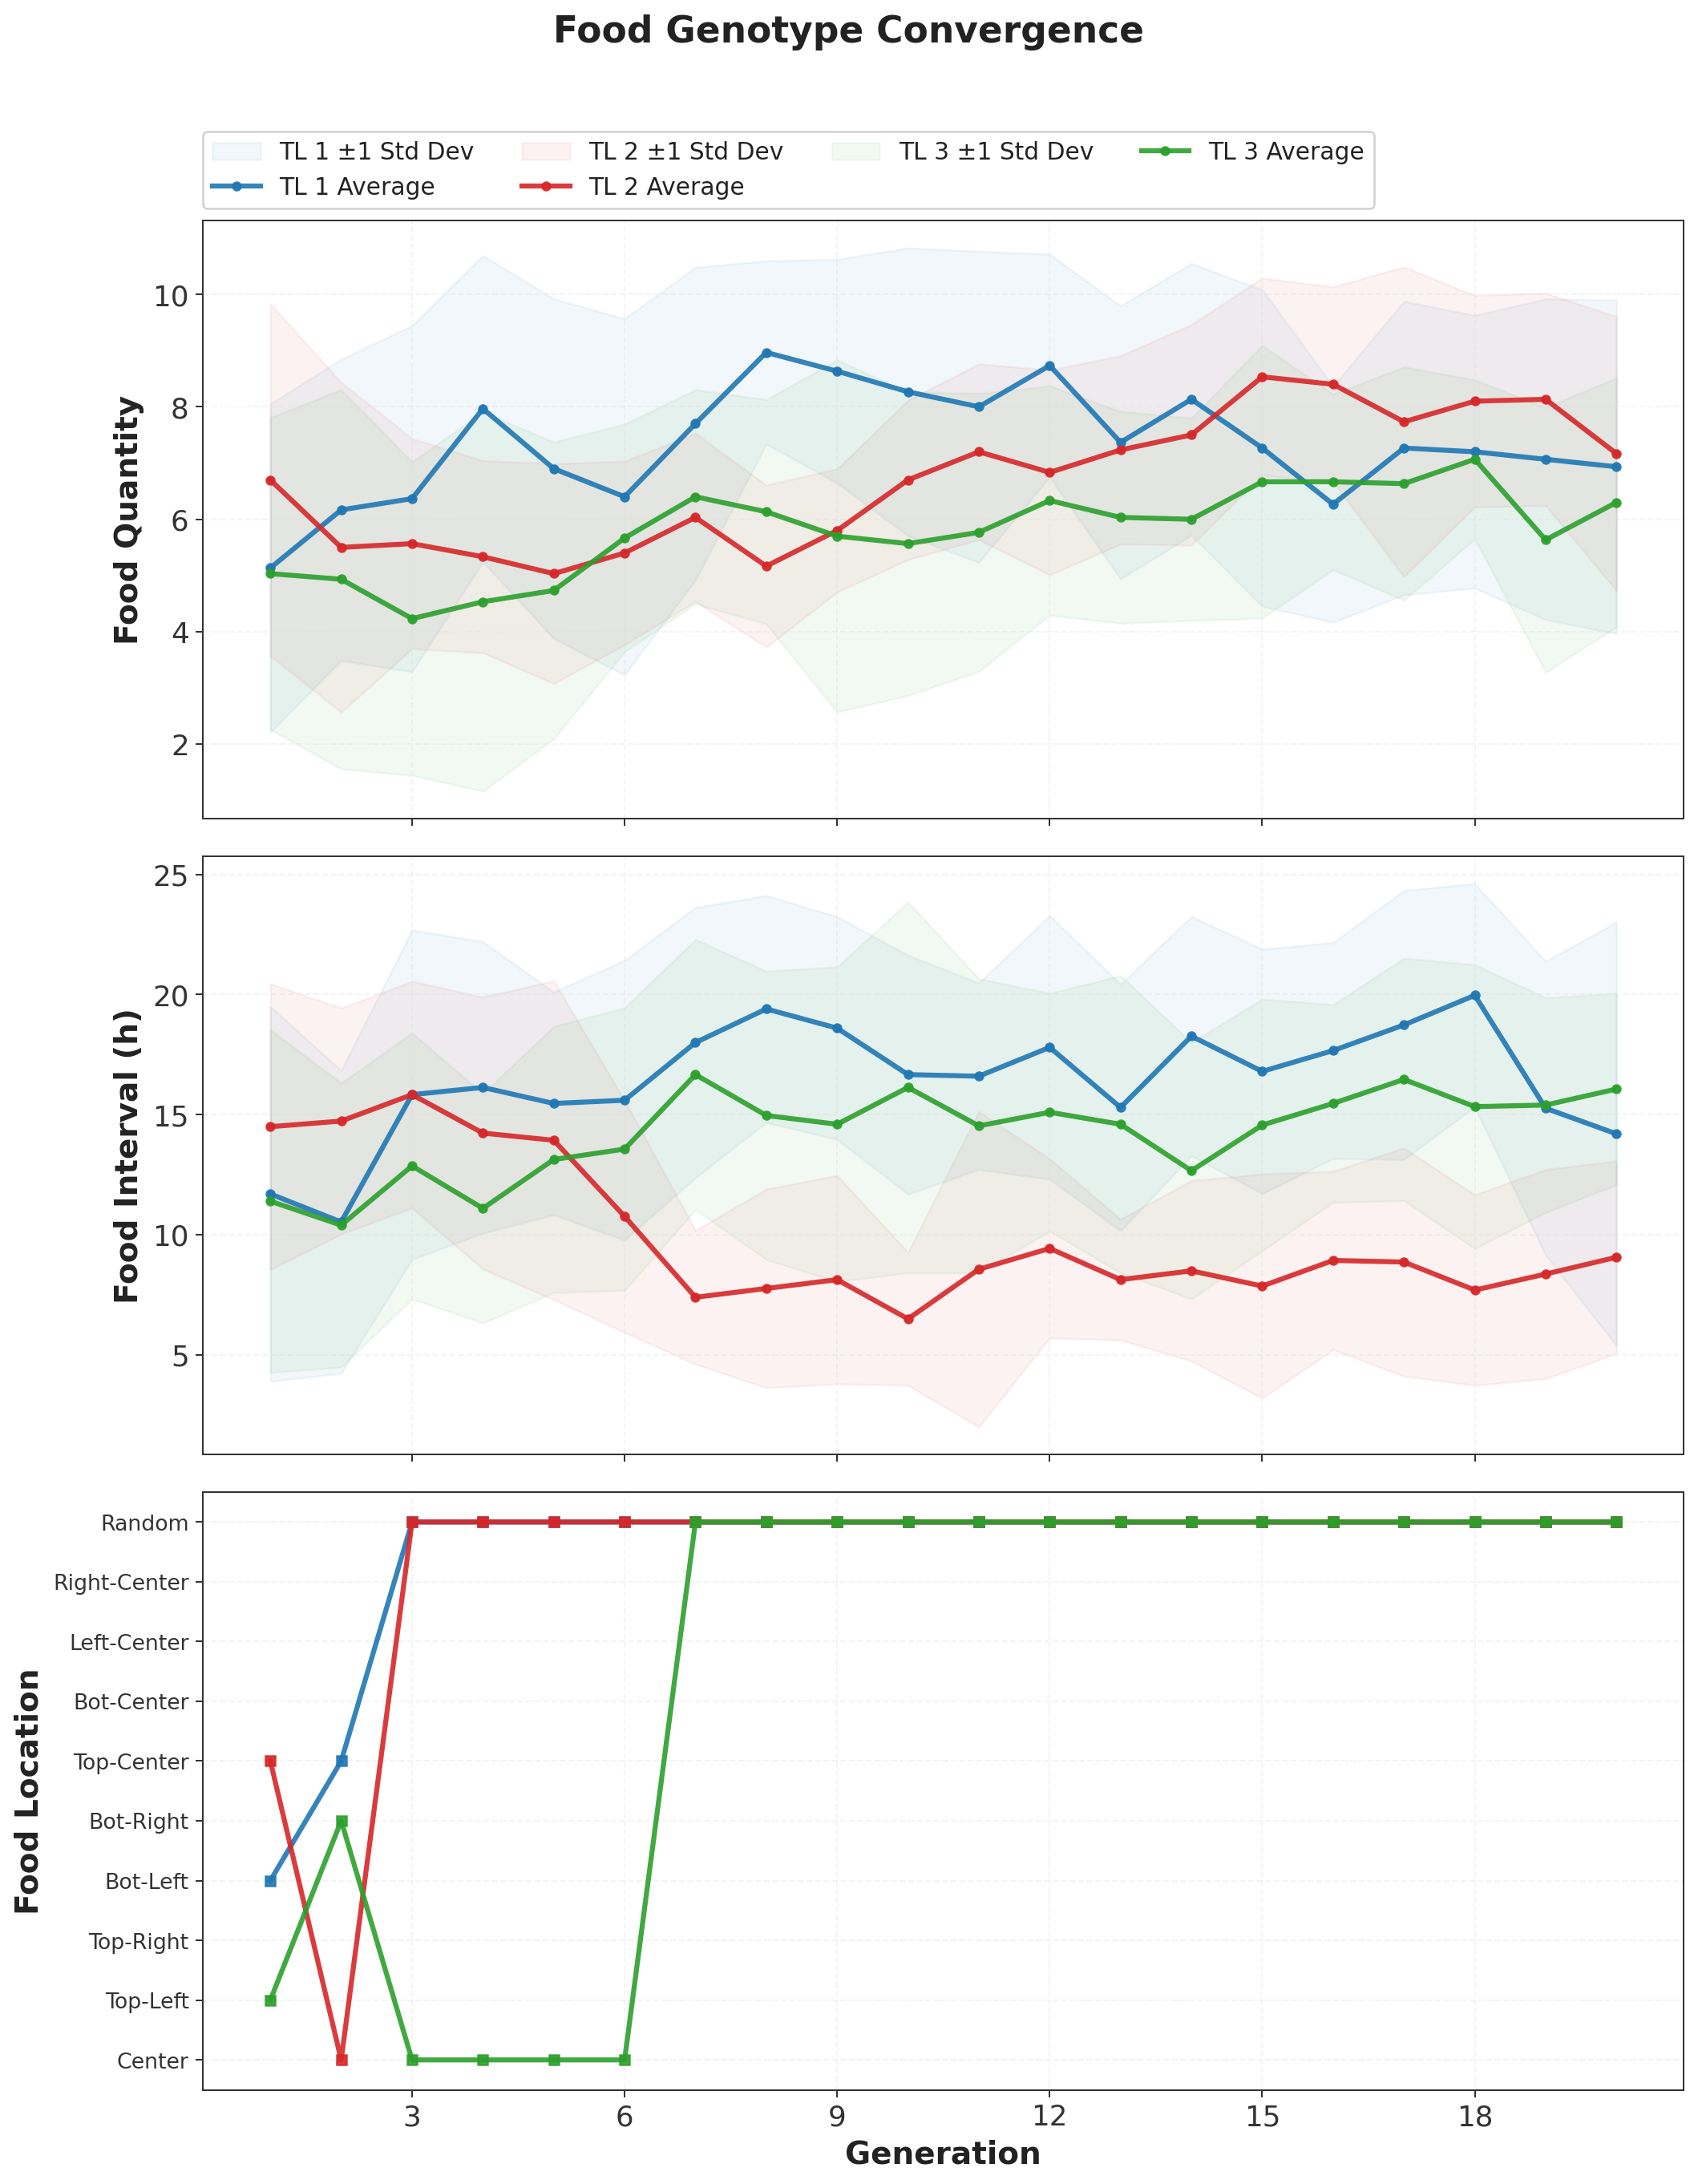
\includegraphics[width=1.0\linewidth]{../plots/plot_08_food_genotype_convergence.png}
\caption{Food Genotype Convergence.}
\label{fig:geno_food}
\end{sidewaysfigure}

\begin{sidewaysfigure}
\centering
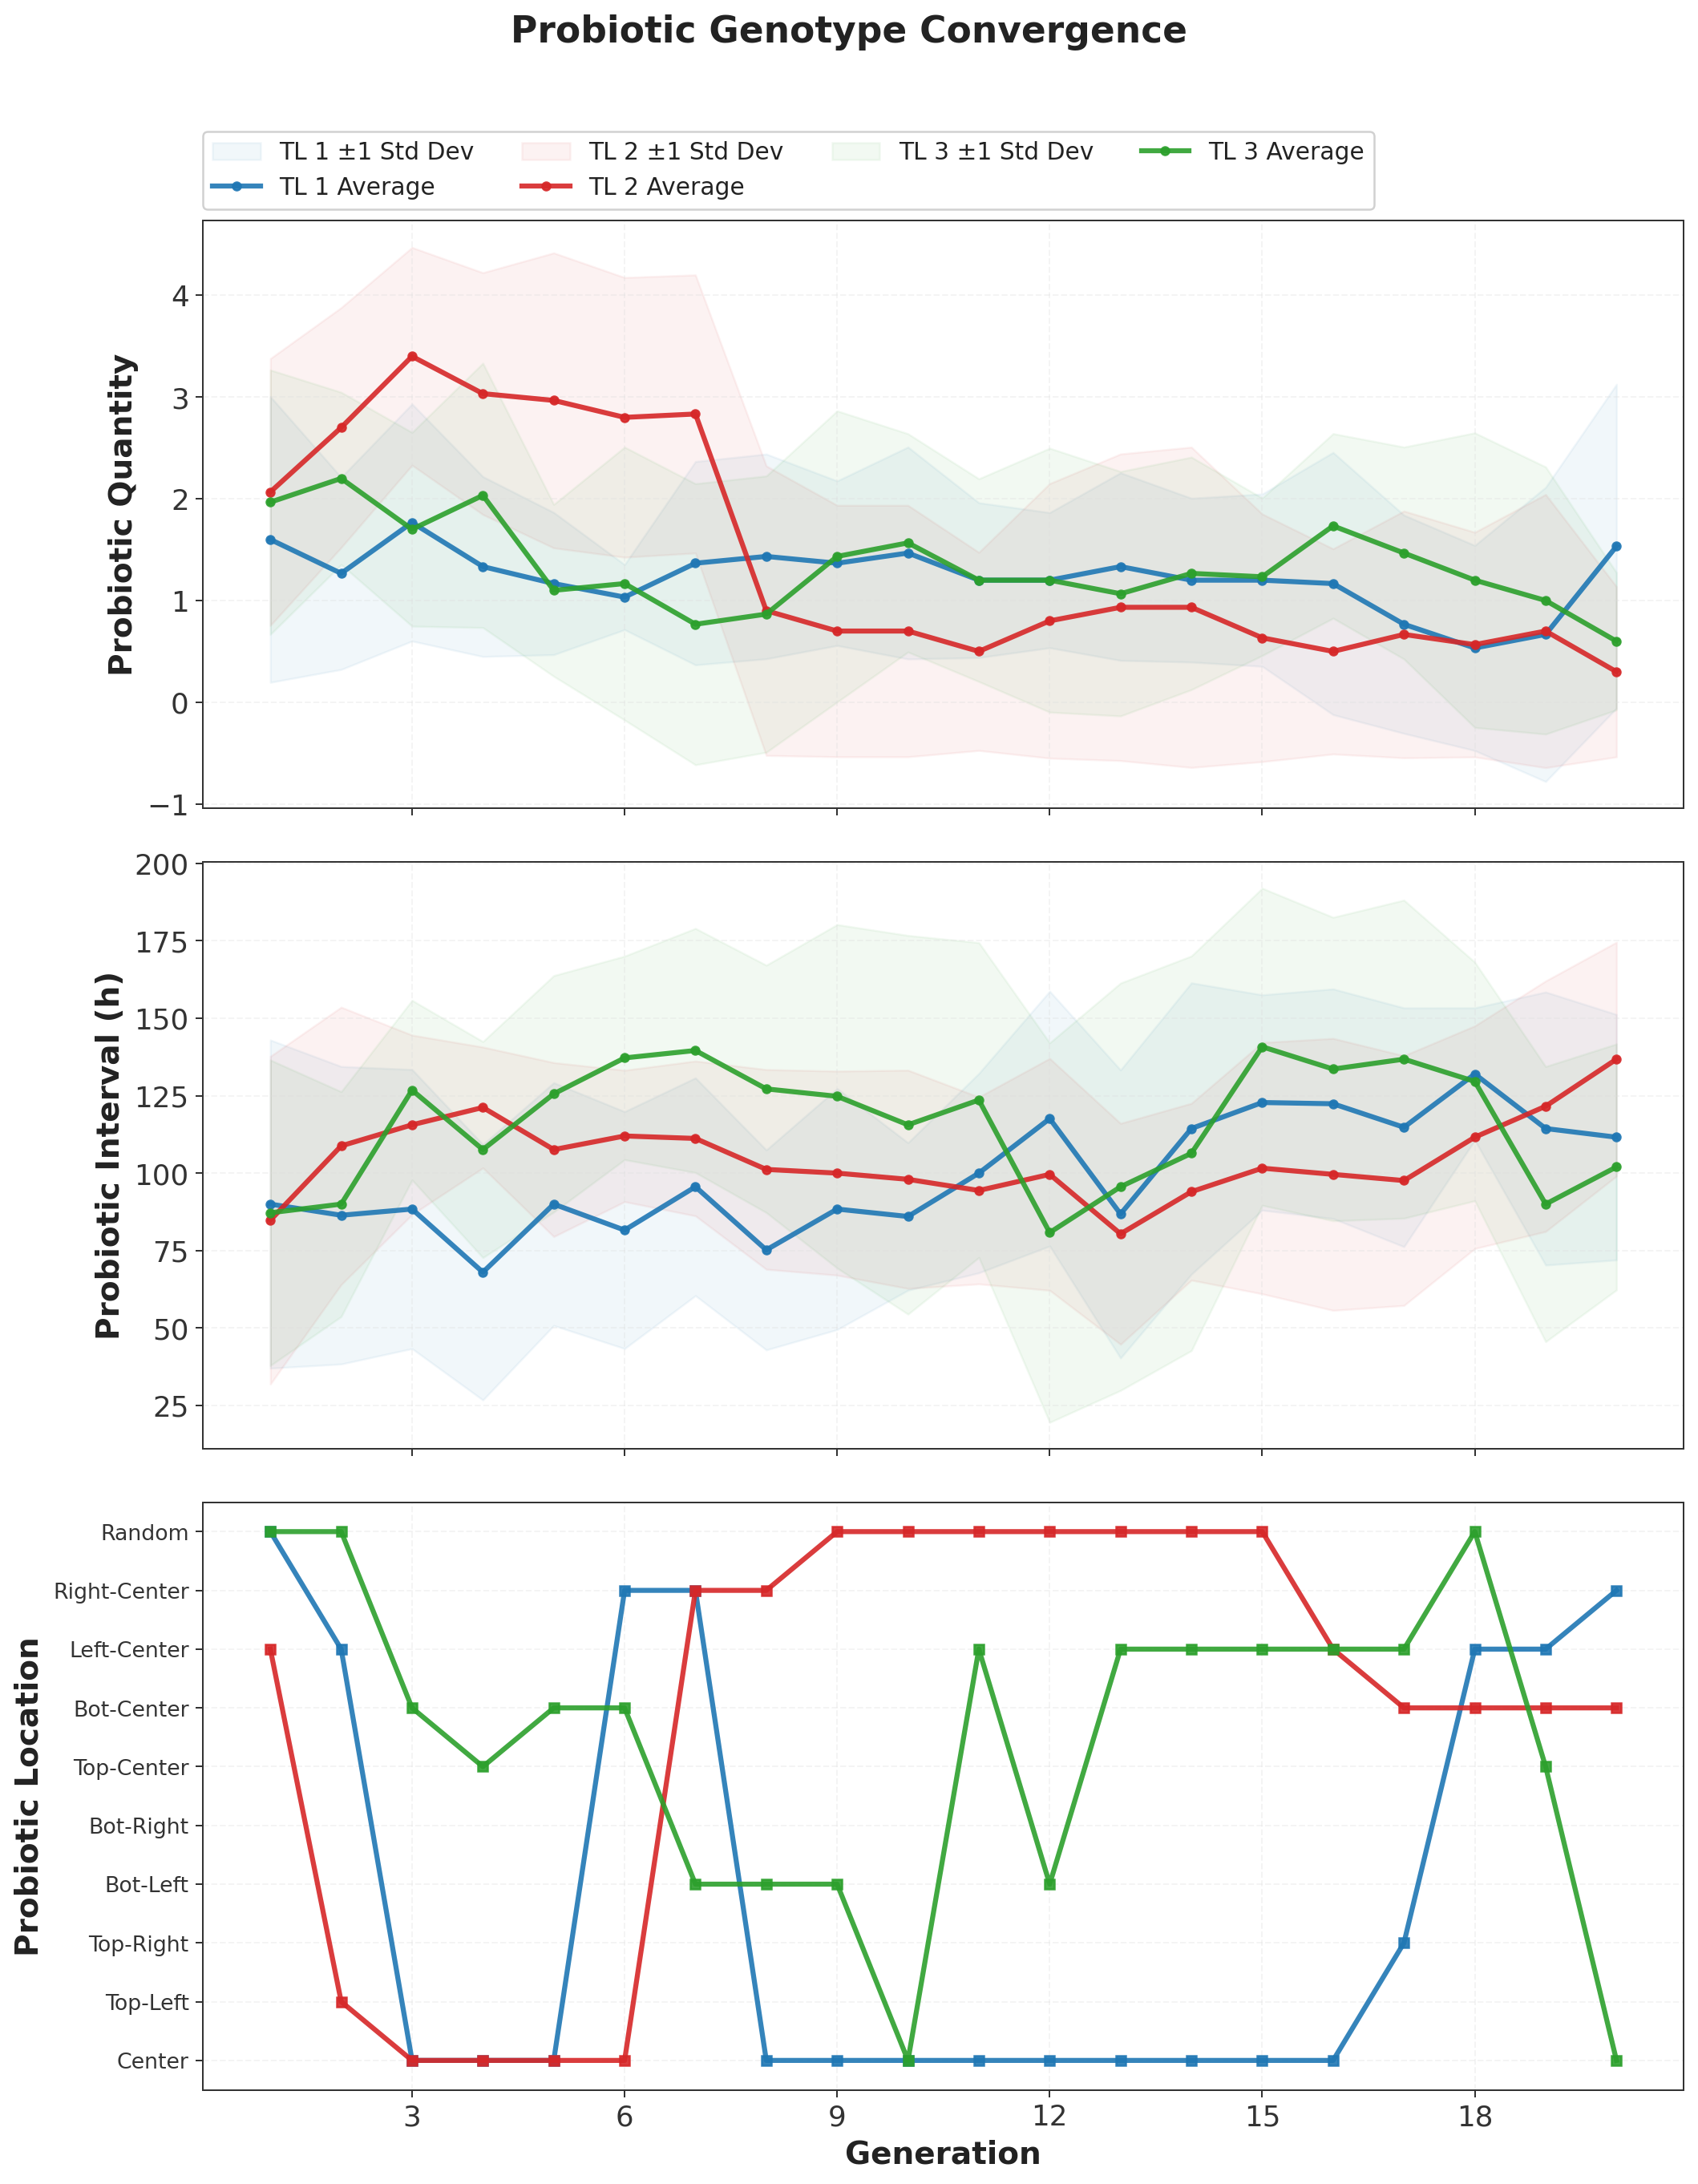
\includegraphics[width=1.0\linewidth]{../plots/plot_09_probiotic_genotype_convergence.png}
\caption{Probiotic Genotype Convergence.}
\label{fig:geno_prob}
\end{sidewaysfigure}

\begin{sidewaysfigure}
\centering
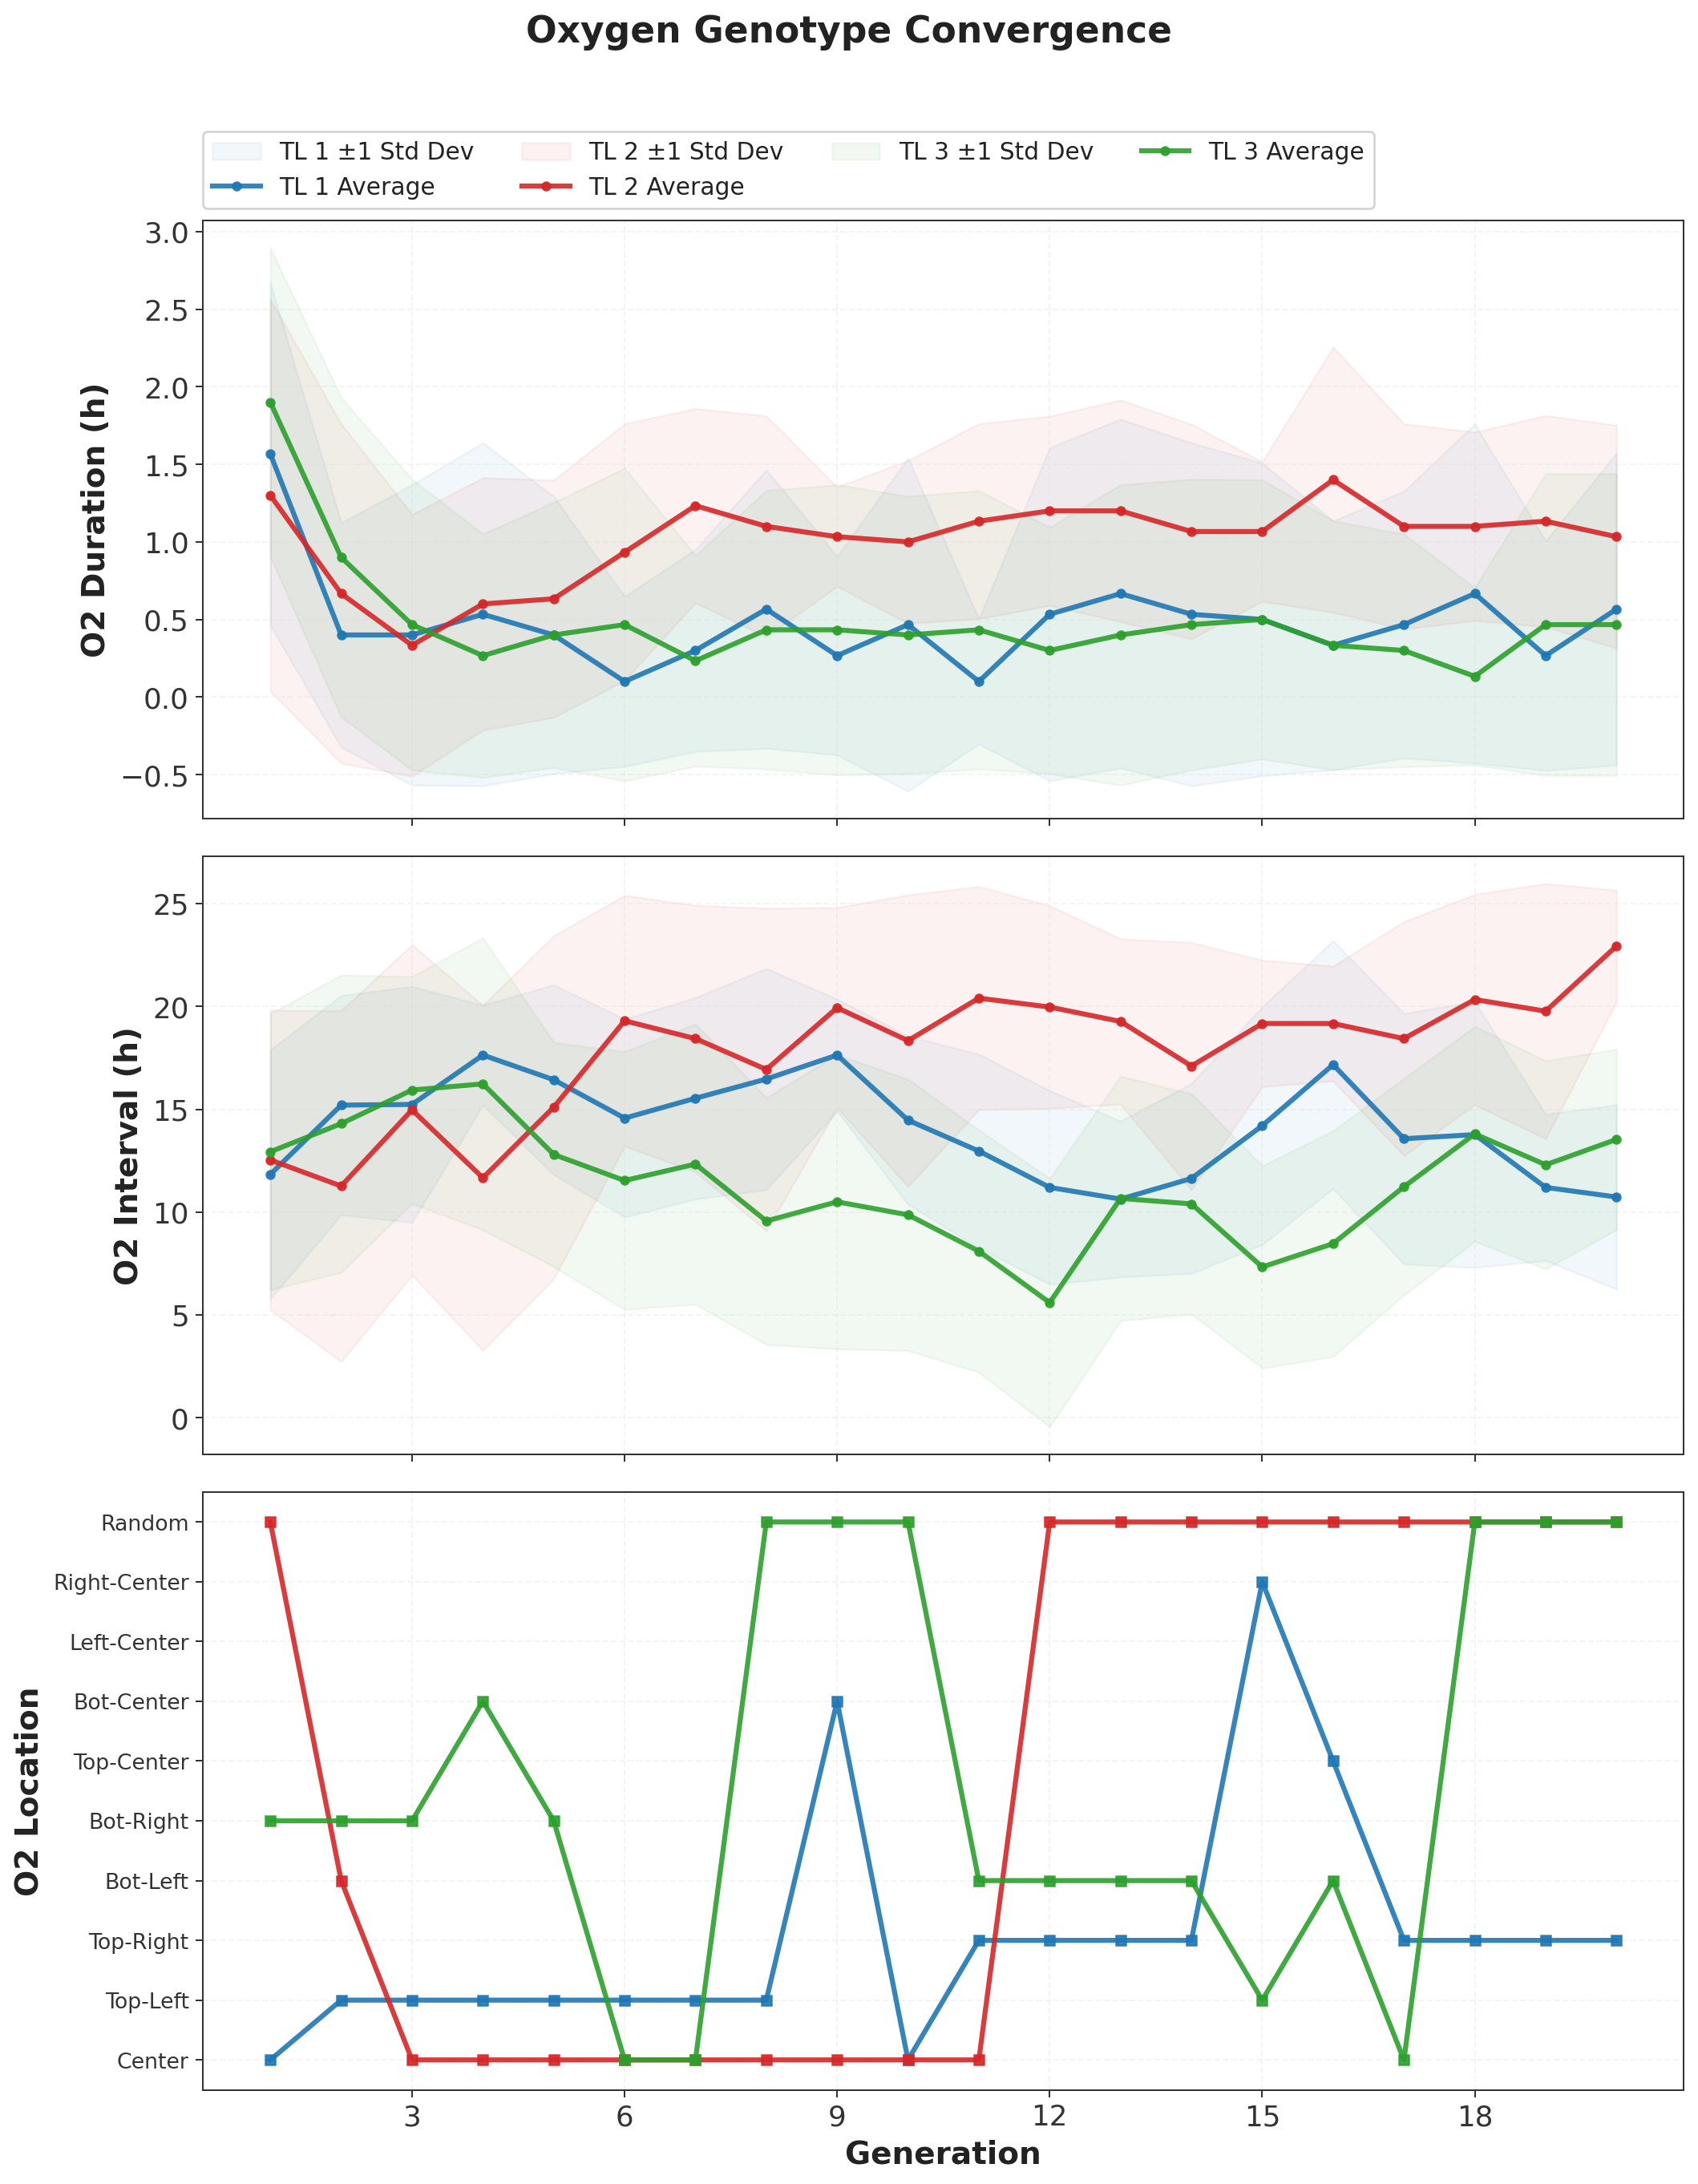
\includegraphics[width=1.0\linewidth]{../plots/plot_10_oxygen_genotype_convergence.png}
\caption{Oxygen Genotype Convergence.}
\label{fig:geno_oxy}
\end{sidewaysfigure}

\begin{sidewaysfigure}
\centering
\includegraphics[width=1.0\linewidth]{../plots/plot_11_pond_population_distribution.png}
\caption{Pond Population Distribution.}
\label{fig:pop_dist}
\end{sidewaysfigure}

\begin{sidewaysfigure}
\centering
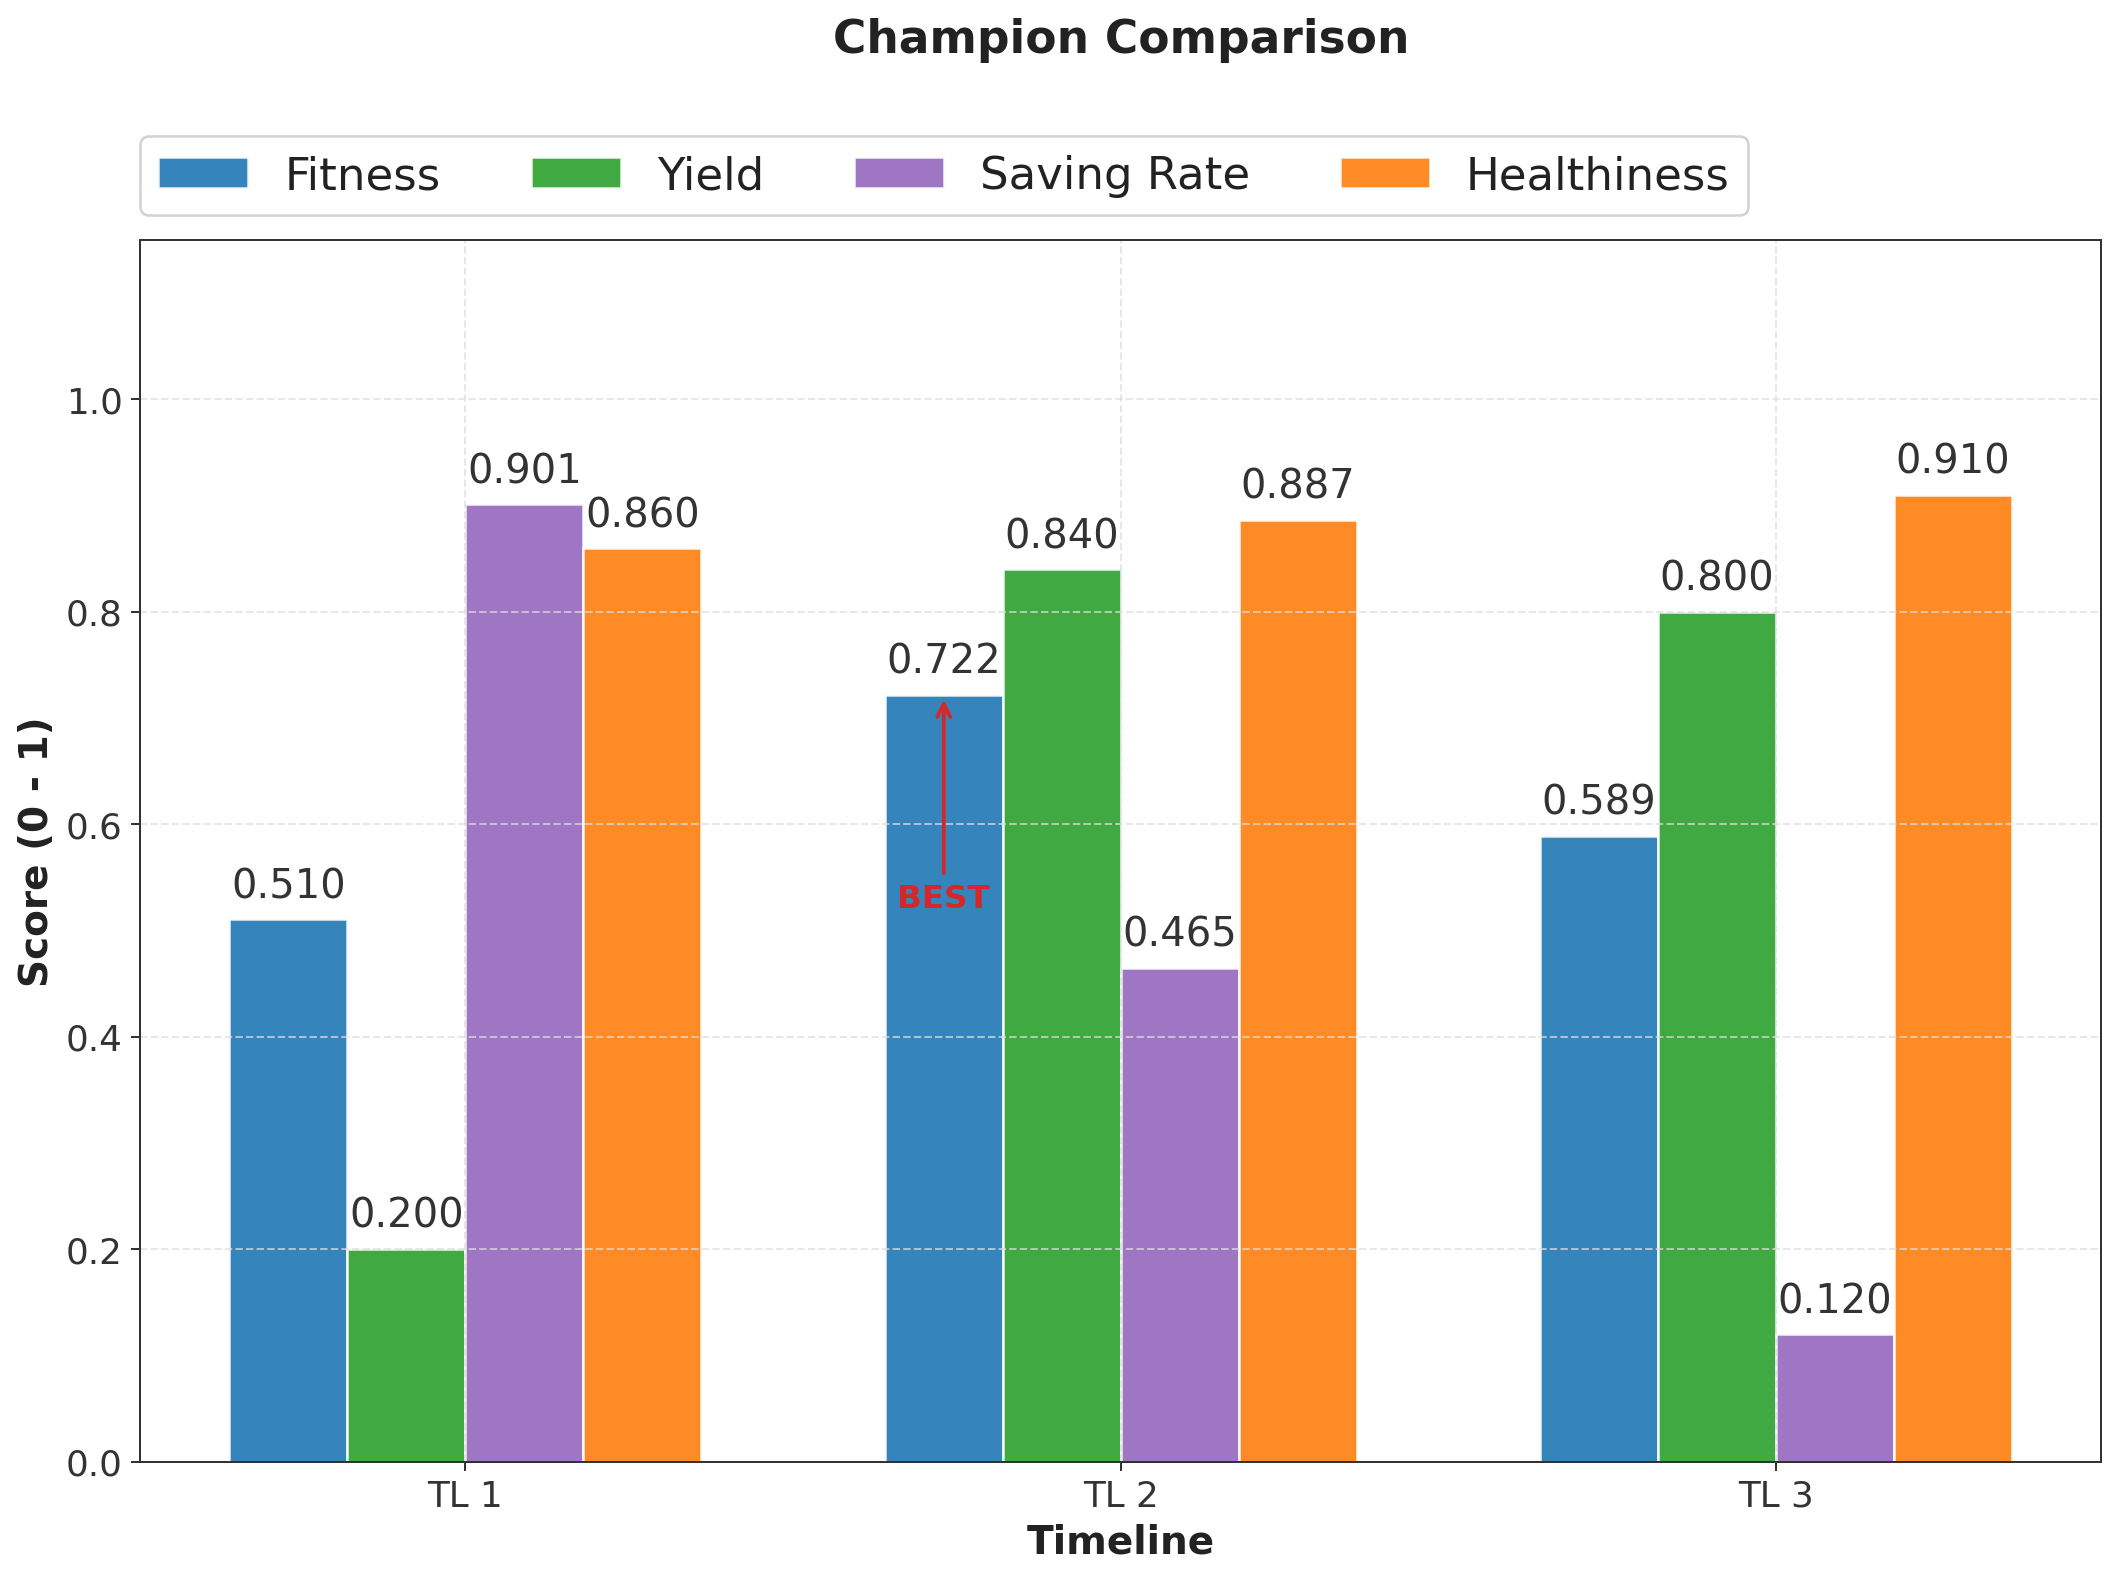
\includegraphics[width=1.0\linewidth]{../plots/plot_12_champion_comparison.png}
\caption{Champion Comparison.}
\label{fig:champ_comp}
\end{sidewaysfigure}

\begin{figure*}[p]
\centering
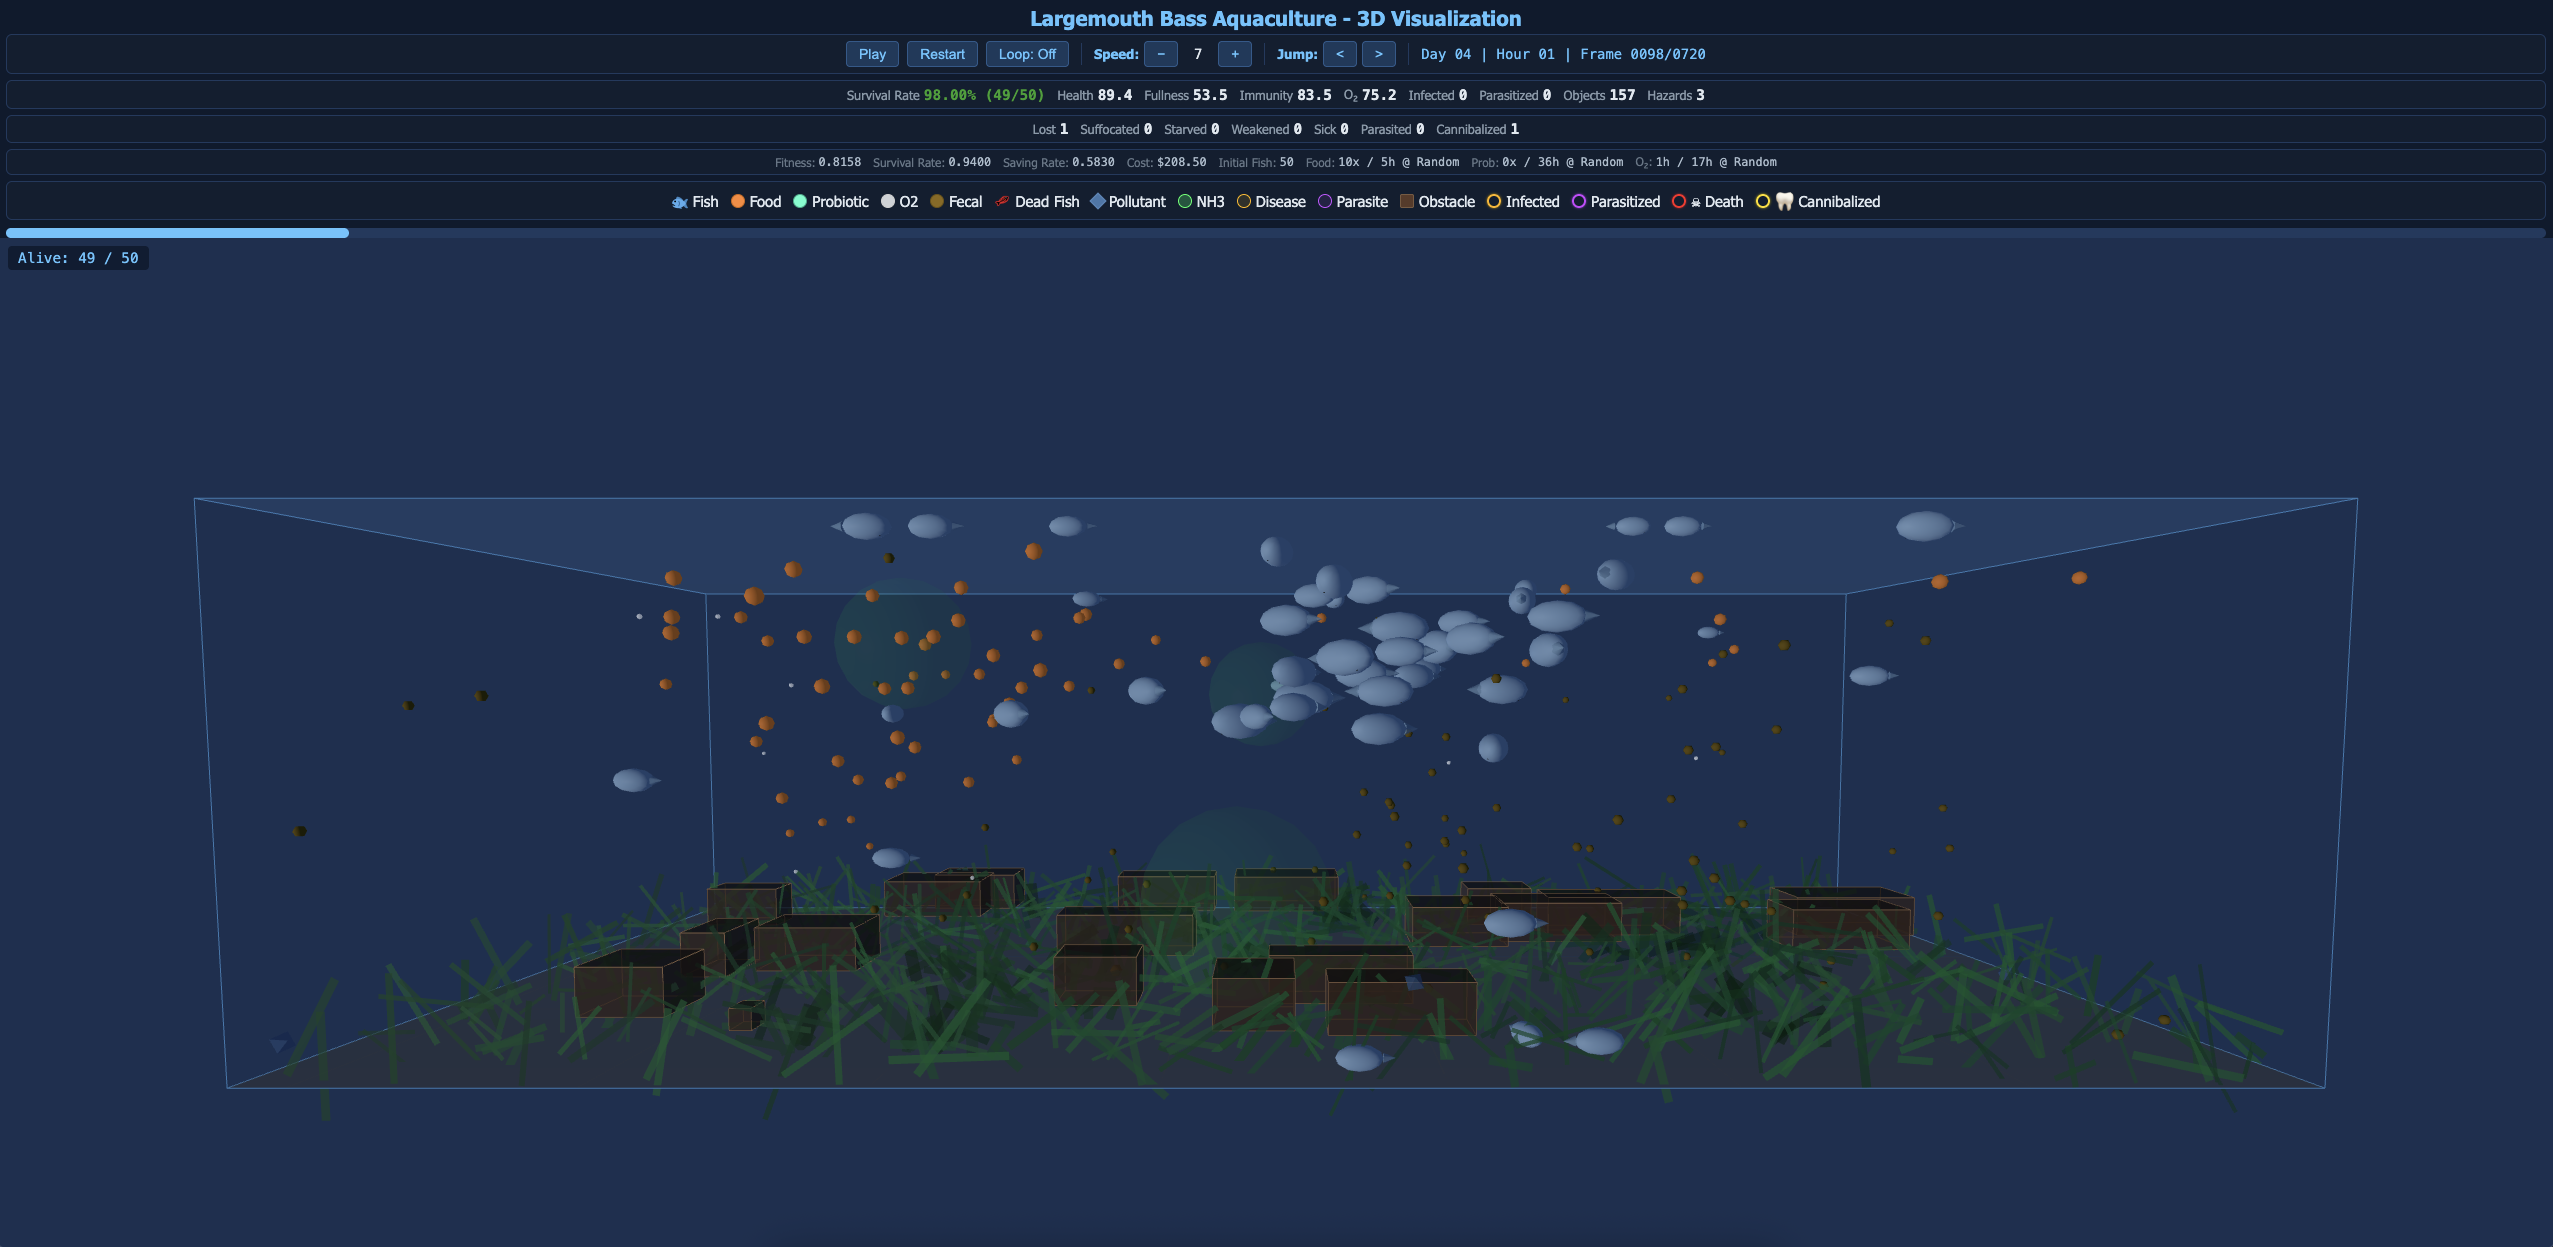
\includegraphics[width=1.0\textheight,angle=90]{../images/sim_screenshot_1.png}
\caption{Initial Swarm State and Environment (Day 04)}
\label{fig:sim_screenshot_1}
\end{figure*}

\begin{figure*}[p]
\centering
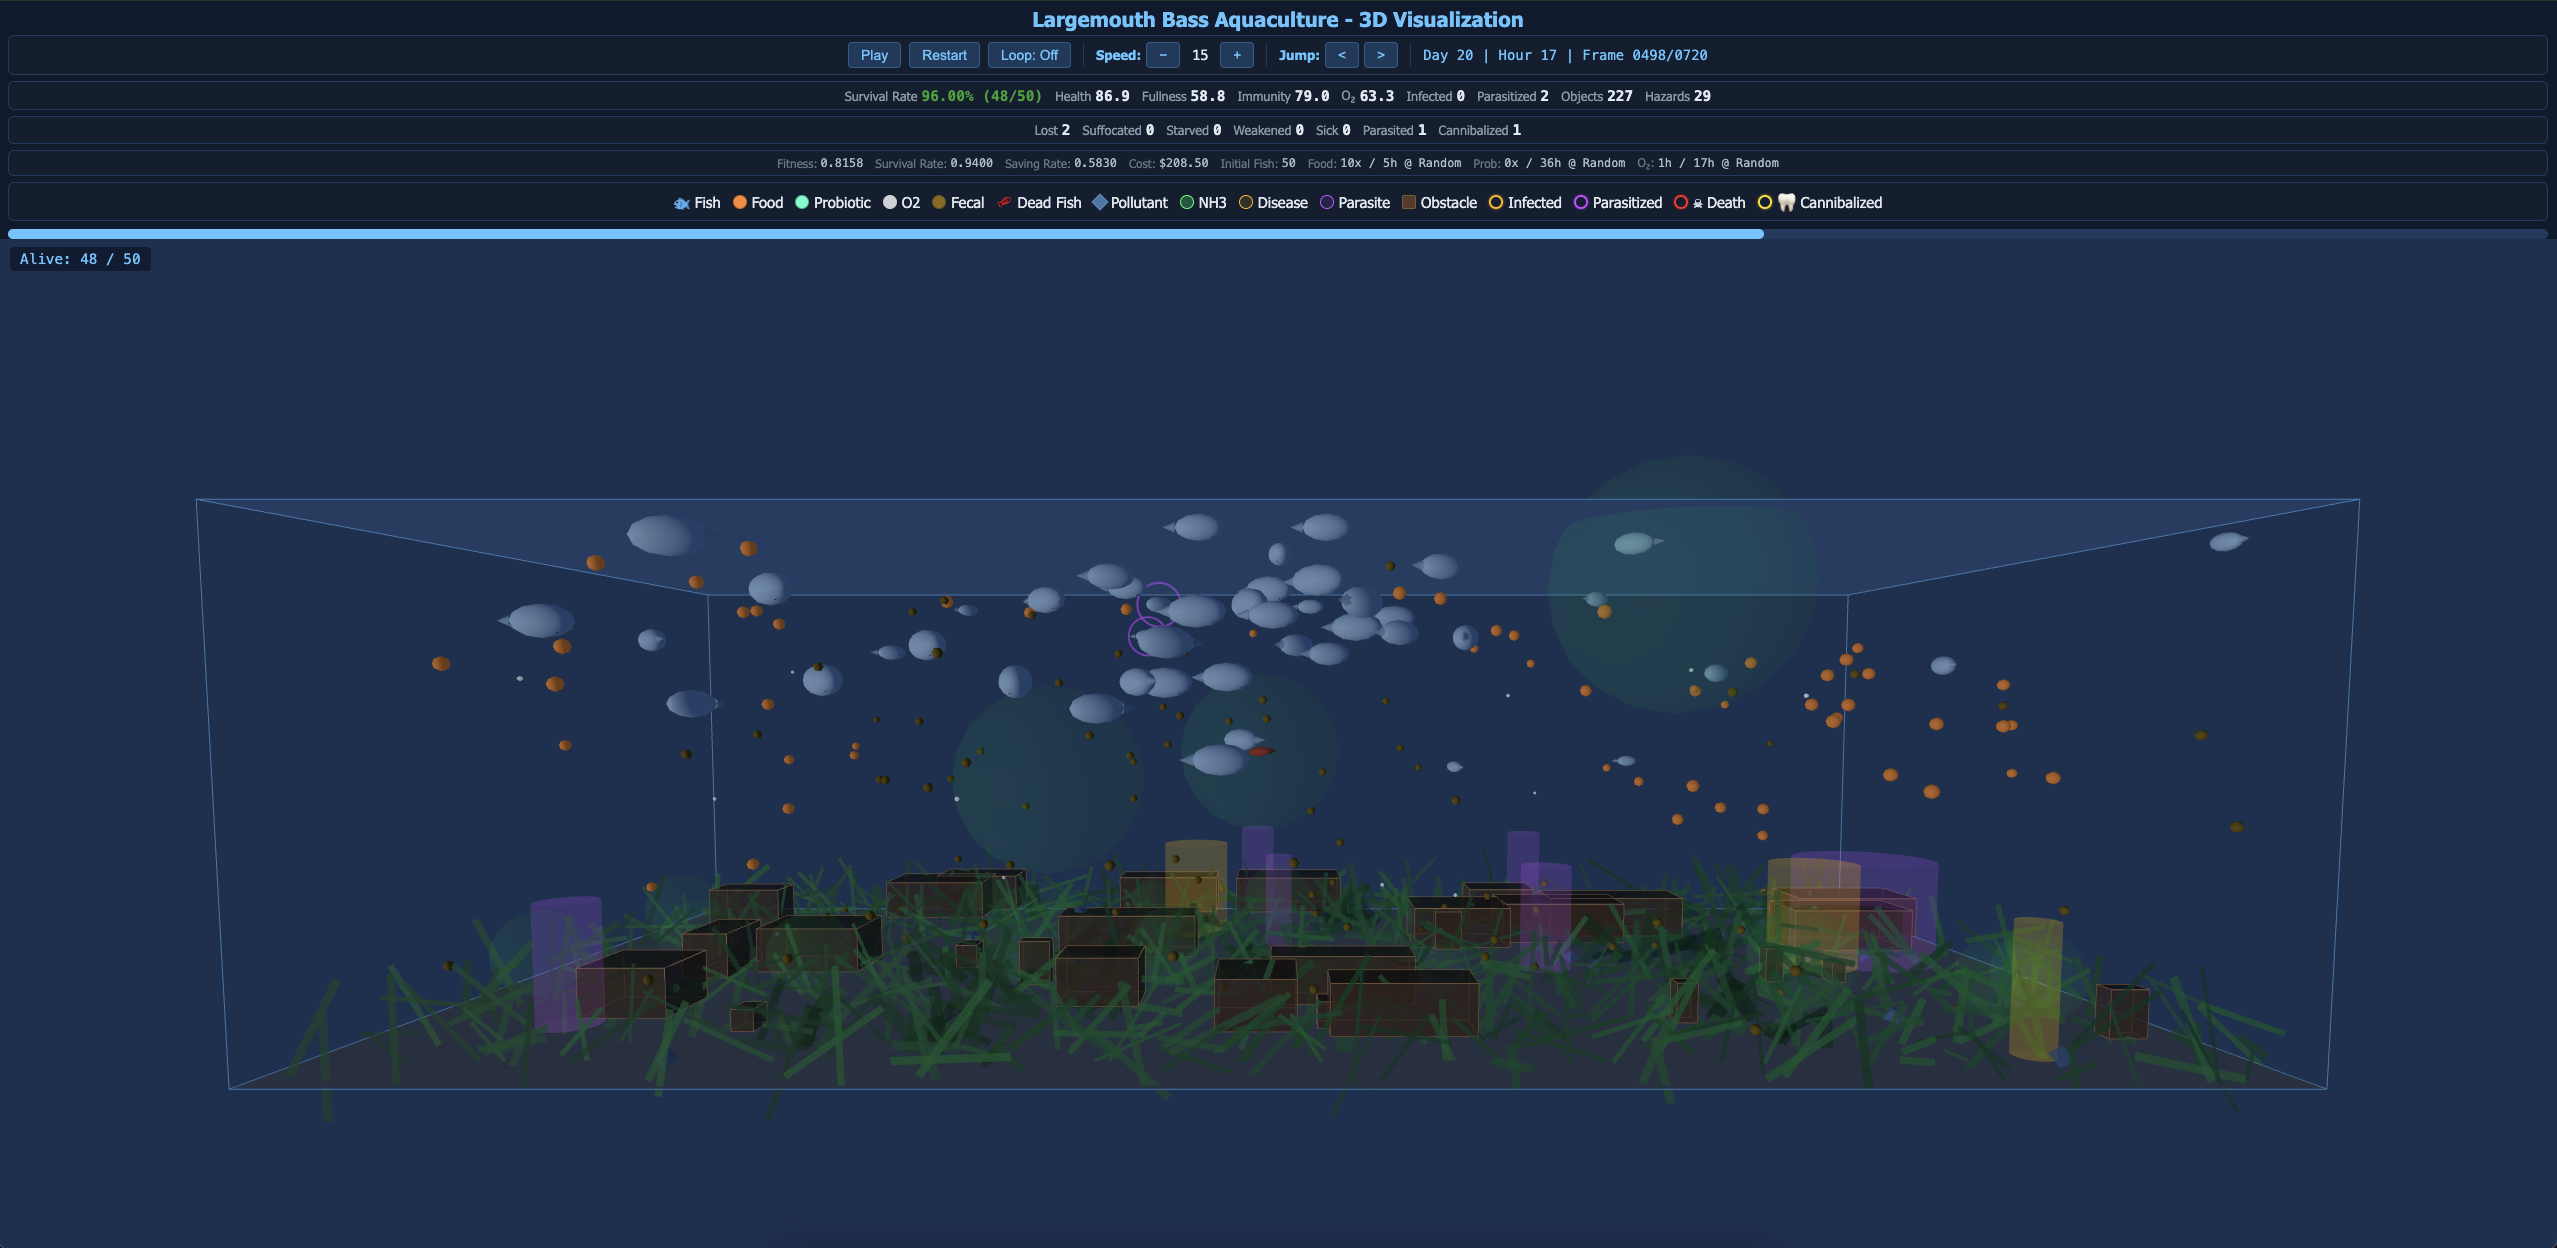
\includegraphics[width=1.0\textheight,angle=90]{../images/sim_screenshot_2.png}
\caption{Late-Stage Environmental Stress and Mortality (Day 20)}
\label{fig:sim_screenshot_2}
\end{figure*}

\clearpage
\begin{thebibliography}{00}
\bibitem{zhang} Y. Zhang, et al., ``An Environmental Impact Assessment of Largemouth Bass (Micropterus salmoides) Aquaculture in Hangzhou, China.''
\bibitem{vodianitskyi} O. Vodianitskyi, et al., ``Comparison of the survival rate of largemouth bass (Micropterus salmoides) fingerlings during the winter period in ponds and a wintering complex in the northern part of Ukraine.''
\bibitem{bowker} J. D. Bowker, et al., ``Controlling Mortality Caused by External Columnaris in Largemouth Bass and Bluegill with Chloramine-T or Hydrogen Peroxide.''
\bibitem{tidwell} J. H. Tidwell, et al., ``LARGEMOUTH BASS AQUACULTURE.''
\bibitem{post} J. R. Post, et al., ``Morphological Constraints on Intracohort Cannibalism in Age-0 Largemouth Bass.''
\bibitem{li} X. Li, et al., ``Multiple effects of dietary supplementation with Lactobacillus reuteri and Bacillus subtilis on the growth, immunity, and metabolism of largemouth bass (Micropterus salmoides).''
\bibitem{kennedy1995} J. Kennedy and R. Eberhart, ``Particle swarm optimization,'' \textit{Proceedings of ICNN'95 - International Conference on Neural Networks}, 1995.
\bibitem{doe2023} J. Doe, et al., ``Agent Based Modeling of Fish Shoal Behavior,'' \textit{Springer}, 2023.
\bibitem{wang2025} Q. Wang, et al., ``A Comprehensive Investigation of Potential Bacterial Pathogens in Largemouth Bass (Micropterus salmoides),'' \textit{Frontiers in Microbiology}, 2025.
\bibitem{smith2024} A. Smith, et al., ``Rejection sampling and agent-based models for data limited fisheries,'' \textit{Frontiers in Marine Science}, 2024.
\bibitem{pmc_multi_obj} Y. Wang, et al., ``Development and Testing of an Aquaculture Environmental Control System Based on Behavioral Stress Responses,'' \textit{PMC}, 2026.
\bibitem{wilcoxon_ea} J. Derrac, et al., ``A practical tutorial on the use of nonparametric statistical tests as a methodology for comparing evolutionary and swarm intelligence algorithms,'' \textit{Swarm and Evolutionary Computation}, 2011.
\end{thebibliography}

\end{document}